% !TeX program = xelatex
\documentclass[11pt,a4paper]{article}

% -------------------------------------------------
% Packages
% -------------------------------------------------
\usepackage{kotex}
\usepackage{fontspec}
\usepackage{amsmath,amssymb,bm,mathtools}
\usepackage[left=24mm,right=24mm,top=23mm,bottom=25mm]{geometry}
\usepackage{booktabs,array}
\usepackage{enumitem}
\usepackage{setspace}
\usepackage{xcolor}
\usepackage{colortbl}
\usepackage{tikz}
\usetikzlibrary{positioning,arrows.meta,calc,fit,decorations.pathreplacing}
\usepackage[most]{tcolorbox}
\usepackage{listings}
\usepackage{hyperref}
\usepackage{fancyhdr}

\setstretch{1.14}
\setlength{\parindent}{0pt}
\setlength{\parskip}{0.55em}

% -------------------------------------------------
% Colors and boxes
% -------------------------------------------------
\definecolor{deepblue}{RGB}{34,71,120}
\definecolor{softblue}{RGB}{239,246,253}
\definecolor{softgray}{RGB}{246,247,249}
\definecolor{softgreen}{RGB}{239,249,242}
\definecolor{softyellow}{RGB}{255,249,229}
\definecolor{codegray}{RGB}{248,248,248}

\newtcolorbox{keybox}[1][]{
  colback=softblue,
  colframe=deepblue,
  boxrule=0.7pt,
  arc=2mm,
  title=#1,
  fonttitle=\bfseries
}

\newtcolorbox{thinkbox}[1][]{
  colback=softyellow,
  colframe=orange!70!black,
  boxrule=0.6pt,
  arc=2mm,
  title=#1,
  fonttitle=\bfseries
}

\newtcolorbox{remarkbox}[1][]{
  colback=softgray,
  colframe=black!45,
  boxrule=0.5pt,
  arc=2mm,
  title=#1,
  fonttitle=\bfseries
}

\newtcolorbox{mlbox}[1][]{
  colback=softgreen,
  colframe=green!45!black,
  boxrule=0.6pt,
  arc=2mm,
  title=#1,
  fonttitle=\bfseries
}

% -------------------------------------------------
% Code style
% -------------------------------------------------
\lstdefinestyle{pythonstyle}{
  language=Python,
  backgroundcolor=\color{codegray},
  basicstyle=\ttfamily\small,
  keywordstyle=\bfseries,
  commentstyle=\itshape\color{black!60},
  stringstyle=\color{black!75},
  numbers=left,
  numberstyle=\tiny\color{black!55},
  numbersep=8pt,
  frame=single,
  rulecolor=\color{black!25},
  breaklines=true,
  showstringspaces=false,
  tabsize=4,
  columns=fullflexible,
  keepspaces=true
}
\lstset{style=pythonstyle}

% -------------------------------------------------
% Math commands
% -------------------------------------------------
\newcommand{\R}{\mathbb{R}}
\newcommand{\grad}{\nabla}
\newcommand{\vect}[1]{\bm{#1}}
\newcommand{\T}{^{\mathsf T}}
\newcommand{\loss}{\mathcal{L}}
\newcommand{\sigmoid}{\sigma}
\newcommand{\pd}[2]{\frac{\partial #1}{\partial #2}}
\newcommand{\softmax}{\operatorname{softmax}}

% -------------------------------------------------
% Header / footer
% -------------------------------------------------
\pagestyle{fancy}
\fancyhf{}
\lhead{Introduction to Deep Learning and Practice}
\rhead{Multi-class Classification}
\cfoot{\thepage}
\renewcommand{\headrulewidth}{0.4pt}
\setlength{\headheight}{14pt}

\hypersetup{
  colorlinks=true,
  linkcolor=deepblue,
  urlcolor=deepblue
}

% =================================================
\begin{document}
% =================================================

\begin{center}
{\LARGE\bfseries 다차원 다중분류와 Softmax, Cross Entropy loss}\\[0.35em]
{\Large Affine $\rightarrow$ Activation $\rightarrow$ Softmax $\rightarrow$ Cross Entropy
$\rightarrow$ Mini-batch $\rightarrow$ MNIST}\\[0.8em]
\end{center}

\vspace{0.4em}

\begin{keybox}[이번 주의 핵심 질문]
지난주에는 입력 $x$ 하나, 출력 $\widehat y$ 하나인 network를 MSE로 학습하였다.
그러나 실제 문제에서는
\begin{itemize}[leftmargin=1.8em]
\item 입력이 \textbf{여러 개의 변수}로 이루어진다.
(예: $28\times28$ 손글씨 이미지 $\Rightarrow$ $784$개의 픽셀 값)
\item 정답이 \textbf{여러 개의 class} 중 하나이다.
(예: 숫자 $0,1,\ldots,9$ $\Rightarrow$ $10$개의 class)
\end{itemize}
그렇다면 network의 출력을 어떻게 ``각 class일 확률''로 바꾸고,
어떤 손실함수로 학습하며,
행렬로 된 parameter의 gradient는 어떻게 계산할까?
그리고 $60000$개나 되는 데이터를 어떻게 효율적으로 학습시킬까?
\end{keybox}

\subsection*{학습목표}

이 주차가 끝나면 다음을 설명하고 직접 계산할 수 있어야 한다.

\begin{enumerate}[label=\arabic*.]
\item 다차원 다중분류 network의 각 변수와 parameter의 shape을 말할 수 있다.
\item affine 계층 $A=XW+B$의 역전파 $\pd{l}{X}$, $\pd{l}{W}$, $\pd{l}{B}$를 성분 계산으로부터 유도한다.
\item sigmoid와 ReLU 활성화 계층의 역전파를 성분별 곱으로 쓸 수 있다.
\item 정답을 one-hot vector로 나타내고, 출력 점수를 softmax로 확률분포로 바꾸는 이유를 설명한다.
\item 두 확률분포를 비교하는 cross entropy 손실함수를 이해한다.
\item softmax와 cross entropy를 묶은 계층의 역전파가 $Y-t$임을 유도한다.
\item mini-batch 학습에서 평균 손실의 gradient를 행렬곱과 \texttt{np.sum}으로 계산한다.
\item NumPy만으로 MNIST 손글씨 숫자 분류 network를 구현하고 학습시킨다.
\end{enumerate}

% =================================================
\section{다차원 다중분류 문제와 신경망의 구조}
% =================================================

\subsection{문제 설정}

$l$차원의 입력 변수
\[
X_{1\times l}=(x_1,x_2,\ldots,x_l)
\]
를 $n$개의 class $\{1,2,\ldots,n\}$ 중 하나로 분류하는 문제를 생각하자.

\begin{itemize}[leftmargin=1.8em]
\item 입력 변수의 차원이 $l>1$인 경우를 \textbf{다차원} 문제라 한다.
\item class의 수가 $n=2$이면 \textbf{이진분류(binary classification)},
$n>2$이면 \textbf{다중분류(multi-class classification)}라 한다.
\end{itemize}

이번 주에 다룰 다차원 다중분류의 대표적인 예가 \textbf{MNIST 손글씨 숫자 데이터}이다.
MNIST는 사람들이 손으로 쓴 숫자 $0\sim9$의 흑백 이미지
$70000$장(훈련용 $60000$장, test용 $10000$장)으로 이루어져 있다.

\IfFileExists{figures/mnist_grid.png}{%
\begin{center}
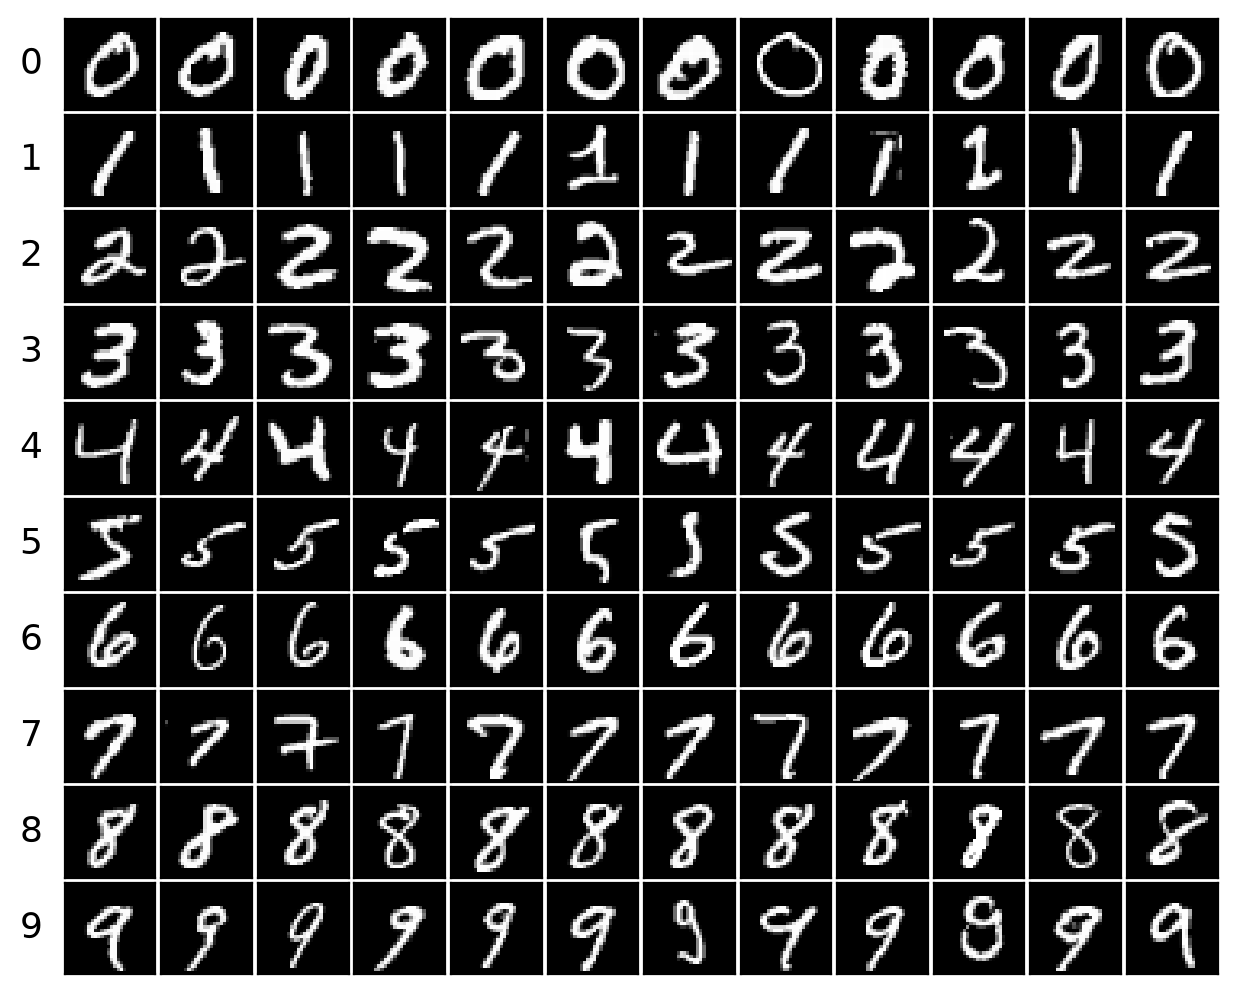
\includegraphics[width=0.78\textwidth]{figures/mnist_grid.png}

\small MNIST 훈련 데이터의 예. 각 행은 class $0,1,\ldots,9$이며,
같은 숫자도 쓰는 사람에 따라 모양이 매우 다양하다.
\end{center}
}{%
\begin{center}
\fbox{\parbox{0.8\textwidth}{\centering\small
[그림 자리] \texttt{figures/mnist\_grid.png}\\
\texttt{mnist\_intro\_figures.py}를 실행하면 생성된다.}}
\end{center}
}

각 이미지는 $28\times28=784$개의 픽셀로 되어 있고,
각 픽셀은 밝기를 나타내는 $0$(검정)$\sim255$(흰색)의 정수이다.
이 $784$개의 픽셀 값을 첫 번째 줄부터 차례로 \textbf{한 줄로 늘어놓으면}
하나의 행벡터
\[
X_{1\times784}=(x_1,x_2,\ldots,x_{784})
\]
가 되고, 이것이 network에 들어가는 \textbf{하나의 훈련 데이터(training example)}이다.
각 이미지의 첫 번째 줄이 $x_1\sim x_{28}$, 두 번째 줄이 $x_{29}\sim x_{56}$, $\ldots$,
마지막 줄이 $x_{757}\sim x_{784}$가 된다.

\IfFileExists{figures/mnist_flatten.png}{%
\begin{center}
\begin{minipage}{\textwidth}
\centering
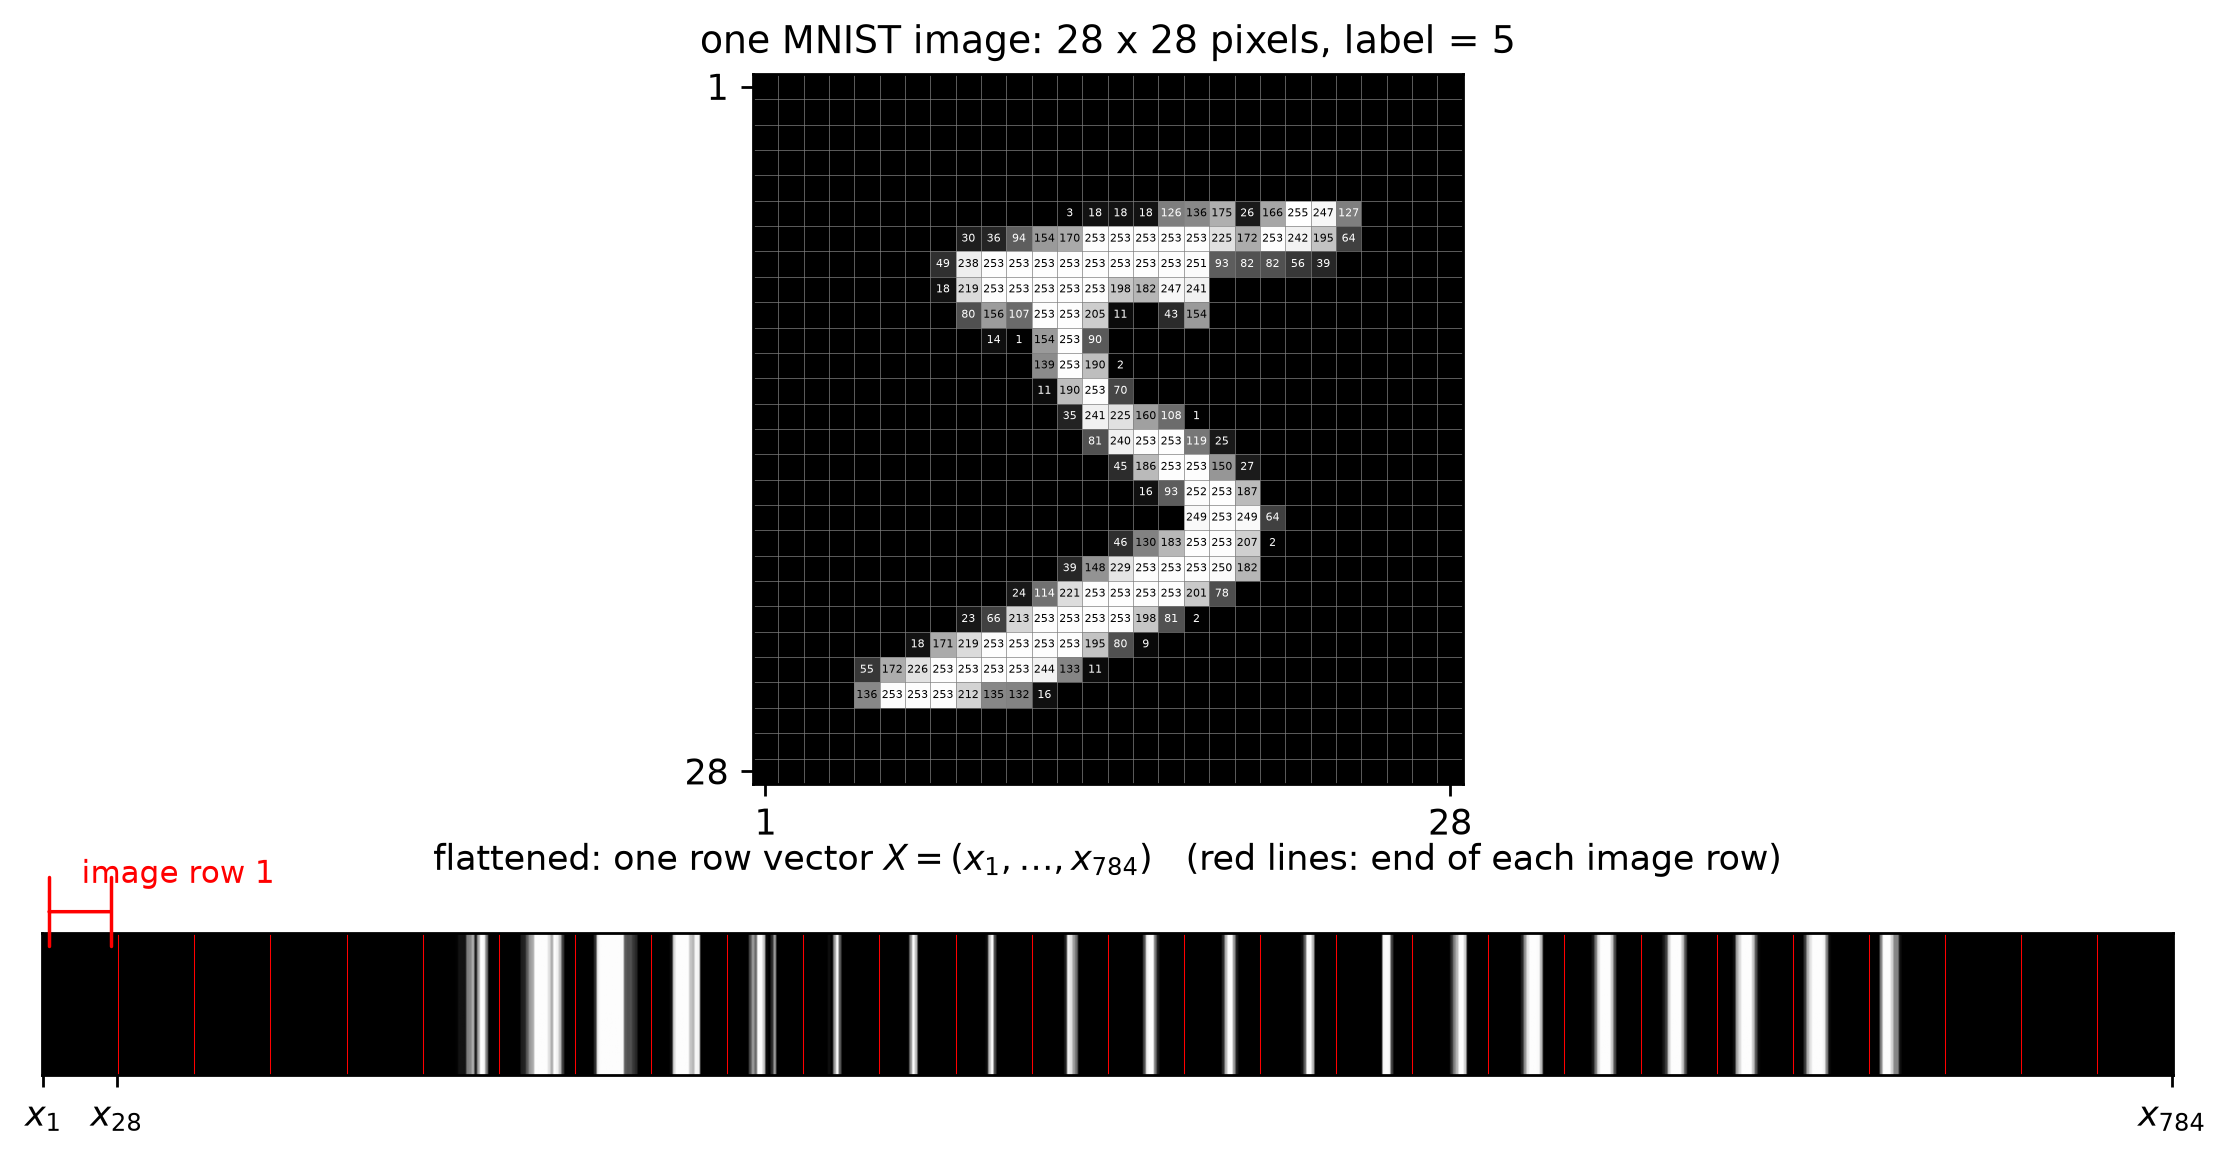
\includegraphics[width=0.74\textwidth]{figures/mnist_flatten.png}

\small 하나의 MNIST 이미지(정답 label $=5$)와 그 픽셀 값(위),
그리고 이를 한 줄로 펼친 $1\times784$ 행벡터(아래).
빨간 선은 이미지의 각 줄이 끝나는 위치이다.
\end{minipage}
\end{center}
}{%
\begin{center}
\fbox{\parbox{0.8\textwidth}{\centering\small
[그림 자리] \texttt{figures/mnist\_flatten.png}\\
\texttt{mnist\_intro\_figures.py}를 실행하면 생성된다.}}
\end{center}
}

정답(label)은 이미지가 나타내는 숫자이므로 class는
\[
\{0,1,2,\ldots,9\}\qquad(n=10)
\]
의 $10$개이다. 즉 MNIST 분류는
\textbf{$l=784$차원의 입력을 $n=10$개의 class 중 하나로 분류하는 다차원 다중분류 문제}이다.
($0,\ldots,9$의 label을 class $1,\ldots,10$으로 번호만 바꿔 생각하면 된다.)

\subsection{신경망의 구조}

은닉층 하나와 softmax 출력층으로 구성된 다음 network를 생각하자.

\begin{center}
\begin{tikzpicture}[>=Latex,
  nd/.style={draw,circle,minimum size=7.5mm,inner sep=0pt,font=\small},
  lab/.style={font=\small}]
% input
\node[nd] (x1) at (0,1.8) {$x_1$};
\node[nd] (x2) at (0,0.8) {$x_2$};
\node at (0,-0.1) {$\vdots$};
\node[nd] (xl) at (0,-1.1) {$x_l$};
% hidden
\node[nd] (a1) at (2.5,1.8) {$a_1$};
\node[nd] (a2) at (2.5,0.8) {$a_2$};
\node at (2.5,-0.1) {$\vdots$};
\node[nd] (am) at (2.5,-1.1) {$a_m$};
\node[nd] (z1) at (3.6,1.8) {$z_1$};
\node[nd] (z2) at (3.6,0.8) {$z_2$};
\node at (3.6,-0.1) {$\vdots$};
\node[nd] (zm) at (3.6,-1.1) {$z_m$};
% output scores
\node[nd] (u1) at (6.1,1.8) {$u_1$};
\node[nd] (u2) at (6.1,0.8) {$u_2$};
\node at (6.1,-0.1) {$\vdots$};
\node[nd] (un) at (6.1,-1.1) {$u_n$};
% softmax
\node[nd] (y1) at (8.3,1.8) {$y_1$};
\node[nd] (y2) at (8.3,0.8) {$y_2$};
\node at (8.3,-0.1) {$\vdots$};
\node[nd] (yn) at (8.3,-1.1) {$y_n$};
% loss
\node[nd] (l) at (10.4,0.35) {$l$};
% edges
\foreach \i in {x1,x2,xl} \foreach \j in {a1,a2,am} \draw[->,black!45] (\i) -- (\j);
\draw[->] (a1) -- (z1); \draw[->] (a2) -- (z2); \draw[->] (am) -- (zm);
\foreach \i in {z1,z2,zm} \foreach \j in {u1,u2,un} \draw[->,black!45] (\i) -- (\j);
\foreach \i in {u1,u2,un} \foreach \j in {y1,y2,yn} \draw[->,orange!70!black!60] (\i) -- (\j);
\foreach \j/\t in {y1/t_1,y2/t_2,yn/t_n} \draw[->,black!60] (\j) -- node[above,font=\scriptsize,sloped] {$\t$} (l);
% labels
\node[lab,red!75!black] at (1.25,2.45) {$W^{(1)},B^{(1)}$};
\node[lab,red!75!black] at (4.85,2.45) {$W^{(2)},B^{(2)}$};
\node[lab,orange!70!black] at (7.2,2.45) {softmax};
\node[lab] at (0,-1.9) {입력층 $X$};
\node[lab,align=center] at (3.05,-1.95) {은닉층\\ $A\to Z=h(A)$};
\node[lab,align=center] at (6.1,-1.95) {출력층\\ (점수) $U$};
\node[lab,align=center] at (8.3,-1.95) {softmax\\ (확률) $Y$};
\node[lab,align=center] at (10.4,-1.95) {손실};
\end{tikzpicture}
\end{center}

입력층의 변수를 $X_{1\times l}$, 은닉층의 변수를 $A_{1\times m}$,
$A$에 활성화 함수 $h$를 적용한 변수를 $Z_{1\times m}$,
출력층의 변수를 $U_{1\times n}$, softmax 함수의 출력을 $Y_{1\times n}$이라 하자.
이 변수들은 가중치 행렬 $W^{(1)}_{l\times m}$, $B^{(1)}_{1\times m}$,
$W^{(2)}_{m\times n}$, $B^{(2)}_{1\times n}$와 활성화 함수 $h$에 의하여
\[
\boxed{
A=XW^{(1)}+B^{(1)},
\qquad
Z=h(A),
\qquad
U=ZW^{(2)}+B^{(2)},
\qquad
Y=\softmax(U)
}
\]
로 정의된다.
은닉층의 node 수는 $m$개이고,
출력층 $U$는 분류하고자 하는 class의 개수와 같은 $n$개의 node를 가진다.
정답을 나타내는 one-hot vector, softmax, 손실함수 $l$은 \ref{sec:onehot}--\ref{sec:smce}절에서 설명한다.

\begin{center}
\begin{tabular}{@{}llll@{}}
\toprule
변수 / parameter & shape & 의미 & MNIST 예 \\
\midrule
$X$ & $1\times l$ & 입력 (한 데이터) & $1\times784$ \\
$W^{(1)},\ B^{(1)}$ & $l\times m,\ 1\times m$ & 첫 번째 affine 계층 & $784\times100,\ 1\times100$ \\
$A,\ Z$ & $1\times m$ & 은닉층 (활성화 전/후) & $1\times100$ \\
$W^{(2)},\ B^{(2)}$ & $m\times n,\ 1\times n$ & 두 번째 affine 계층 & $100\times10,\ 1\times10$ \\
$U$ & $1\times n$ & 각 class의 점수 (score) & $1\times10$ \\
$Y$ & $1\times n$ & 각 class일 확률 & $1\times10$ \\
\bottomrule
\end{tabular}
\end{center}

지난주와 마찬가지로 데이터 하나를 \textbf{행벡터}로 쓰고 $XW$의 순서로 곱한다.
이 규약에서 가중치 행렬의 shape은 항상
\[
\boxed{
W:\ (\text{입력 node 수})\times(\text{출력 node 수})
}
\qquad
\bigl(W^{(1)}:\ l\times m,\quad W^{(2)}:\ m\times n\bigr)
\]
이다. NumPy에서도 \texttt{W1.shape}은 \texttt{(784, 100)}, \texttt{W2.shape}은 \texttt{(100, 10)}이다.
그러면 \ref{sec:minibatch}절에서 데이터(example) $h$개를 행으로 쌓은 행렬 $X_{h\times l}$에 대해서도
\[
\underbrace{X}_{(\text{example 수})\times(\text{입력 node 수})}\
\underbrace{W}_{(\text{입력 node 수})\times(\text{출력 node 수})}
=\underbrace{XW}_{(\text{example 수})\times(\text{출력 node 수})}
\]
이 되어, 같은 식 $XW+B$를 그대로 쓸 수 있다.
결과의 각 \textbf{행}은 각 데이터, 각 \textbf{열}은 다음 층의 각 node에 대응한다.

\begin{remarkbox}[이 network는 몇 층인가? --- 깊이와 넓이]
$A$와 $Z$는 같은 은닉층의 활성화 \textbf{전}과 \textbf{후}의 값이므로 하나의 층으로 센다.
$U$는 class별 점수를 내는 \textbf{출력층}이다.
\begin{itemize}[leftmargin=1.8em]
\item \textbf{깊이(depth)}는 층(layer)의 개수이다.
보통 입력층은 세지 않고, \textbf{가중치를 가진 층}(affine 계층)의 개수를 센다.
위 network는 은닉층 1개와 출력층 1개, 즉 가중치 행렬 $W^{(1)}, W^{(2)}$를 가진 두 층이므로
\textbf{2층 신경망(two-layer network)}이다.
(입력층까지 세어 ``3층''이라 부르는 책도 있으므로, 층을 세는 기준을 확인해야 한다.)
\item \textbf{넓이(width)}는 한 층의 node 수이다.
위 network의 은닉층 넓이는 $m$ (MNIST 예에서는 $100$)이다.
\item 은닉층이 두 개 이상인, 즉 층이 깊은 network를 \textbf{심층신경망(deep neural network)}이라 한다.
\end{itemize}
\end{remarkbox}

\begin{remarkbox}[NumPy 배열의 ``차원''과 벡터의 ``차원'']
NumPy에서 말하는 배열의 차원과 수학에서 말하는 벡터의 차원은 다르다.
\begin{itemize}[leftmargin=1.8em]
\item \texttt{X = np.array([x1, x2, ..., xl])}는 \textbf{1차원 배열}이고
\texttt{X.shape}는 \texttt{(l,)}이다. 수학에서는 원소가 $l$개이므로 $l$차원 벡터라 부른다.
\item \texttt{X = np.array([[x1, x2, ..., xl]])}는 1차원 배열 하나를 원소로 갖는
\textbf{2차원 배열}이고 \texttt{X.shape}는 \texttt{(1, l)}이다.
\end{itemize}
배열의 차원은 \texttt{X.ndim}, 모양은 \texttt{X.shape}로 확인한다.
\begin{lstlisting}
import numpy as np
x = np.array([[1, 2, 3], [4, 5, 6]])
print(x.ndim, x.shape)        # 2 (2, 3)
y = np.array([[[1], [2], [3]], [[4], [5], [6]]])
print(y.ndim, y.shape)        # 3 (2, 3, 1)
\end{lstlisting}
우리는 데이터 하나를 \texttt{(1, l)}, 데이터 $h$개를 \texttt{(h, l)} 모양의 2차원 배열로 다룬다.
\end{remarkbox}

% =================================================
\section{Affine 계층의 역전파 (입력층과 은닉층 사이)}
% =================================================

\subsection{성분으로 쓴 affine 변환}

신경망의 순전파에서 먼저 선형 연결층을 표현해 보자.
편의상 층 번호를 나타내는 위첨자 $(1)$은 생략한다. $A=XW+B$에서
\[
X_{1\times l}=(x_1,\ldots,x_l),
\qquad
A_{1\times m}=(a_1,\ldots,a_m),
\qquad
B_{1\times m}=(b_1,\ldots,b_m),
\]
\[
W_{l\times m}=(w_{ij})=
\begin{pmatrix}
w_{11}&w_{12}&\cdots&w_{1m}\\
w_{21}&w_{22}&\cdots&w_{2m}\\
\vdots&&&\vdots\\
w_{l1}&w_{l2}&\cdots&w_{lm}
\end{pmatrix}
\]
이다.
$A=XW+B$와 같은 일차 변환을 \textbf{affine 변환}이라 하며,
이는 1변수 일차함수 $a=xw+b$를 다변수 벡터함수로 일반화한 것이다.
행렬곱을 전개하여 성분끼리 비교하면
\[
\begin{cases}
a_1=x_1w_{11}+x_2w_{21}+\cdots+x_lw_{l1}+b_1\\
a_2=x_1w_{12}+x_2w_{22}+\cdots+x_lw_{l2}+b_2\\
\qquad\vdots\\
a_m=x_1w_{1m}+x_2w_{2m}+\cdots+x_lw_{lm}+b_m
\end{cases}
\qquad\text{즉}\qquad
\boxed{a_j=\sum_{i=1}^{l}x_iw_{ij}+b_j}
\tag{1}
\]
이다 ($i=1,\ldots,l$, $j=1,\ldots,m$).
가중치 $w_{ij}$는 입력 node $x_i$와 은닉 node $a_j$를 연결하고, $b_j$는 $a_j$에만 연결된다.

\subsection{무엇을 구하려는가}

뒤에서 정의할 손실을 $l$이라 하자.
$A$층까지 어떤 복잡한 계산을 거쳐 역전파된 기울기
\[
\pd{l}{A}=\left(\pd{l}{a_1},\pd{l}{a_2},\ldots,\pd{l}{a_m}\right)_{1\times m}
\]
를 이미 알고 있다고 하자 (뒤쪽 층에서 전달받은 \textbf{upstream gradient}).
목표는
\[
\pd{l}{X}=\left(\pd{l}{x_1},\ldots,\pd{l}{x_l}\right)_{1\times l},
\qquad
\pd{l}{W}=\left(\pd{l}{w_{ij}}\right)_{l\times m},
\qquad
\pd{l}{B}=\left(\pd{l}{b_1},\ldots,\pd{l}{b_m}\right)_{1\times m}
\]
를 $\pd{l}{A}$로 나타내는 것이다.
각 기울기는 해당 변수와 \textbf{같은 shape}을 가진다는 점에 주목하자.

\subsection{$\partial l/\partial X$: 모든 경로의 기여를 더한다}

식 (1)에서 $x_i$는 은닉층의 \textbf{모든} node $a_1,\ldots,a_m$을 거쳐 $l$과 연결되고
$\pd{a_j}{x_i}=w_{ij}$이므로, 합성함수 미분법에 의해
\[
\pd{l}{x_i}
=\sum_{j=1}^{m}\pd{a_j}{x_i}\pd{l}{a_j}
=w_{i1}\pd{l}{a_1}+w_{i2}\pd{l}{a_2}+\cdots+w_{im}\pd{l}{a_m}
=\left(\pd{l}{a_1},\ldots,\pd{l}{a_m}\right)
\begin{pmatrix}w_{i1}\\ \vdots\\ w_{im}\end{pmatrix}
\]
이다. 이를 $i=1,\ldots,l$에 대해 한꺼번에 나타내면
\[
\pd{l}{X}
=\left(\pd{l}{a_1},\ldots,\pd{l}{a_m}\right)
\begin{pmatrix}
w_{11}&w_{21}&\cdots&w_{l1}\\
\vdots&&&\vdots\\
w_{1m}&w_{2m}&\cdots&w_{lm}
\end{pmatrix}
=\pd{l}{A}\,W\T
\]
이다. shape으로 쓰면
$\left(\pd{l}{X}\right)_{1\times l}=\left(\pd{l}{A}\right)_{1\times m}\left(W\T\right)_{m\times l}$이다.

\subsection{$\partial l/\partial W$: 입력과 upstream gradient의 곱}

가중치 $w_{ij}$는 $x_i$와의 곱으로 $a_j$에만 연결되므로
\[
\pd{l}{w_{ij}}=\pd{a_j}{w_{ij}}\pd{l}{a_j}=x_i\pd{l}{a_j}
\]
이다. 행렬로 모두 나타내면
\[
\pd{l}{W}
=
\begin{pmatrix}
x_1\pd{l}{a_1}&x_1\pd{l}{a_2}&\cdots&x_1\pd{l}{a_m}\\[4pt]
x_2\pd{l}{a_1}&x_2\pd{l}{a_2}&\cdots&x_2\pd{l}{a_m}\\
\vdots&&&\vdots\\
x_l\pd{l}{a_1}&x_l\pd{l}{a_2}&\cdots&x_l\pd{l}{a_m}
\end{pmatrix}_{l\times m}
=
\begin{pmatrix}x_1\\ \vdots\\ x_l\end{pmatrix}_{l\times1}
\left(\pd{l}{a_1},\ldots,\pd{l}{a_m}\right)_{1\times m}
=X\T\pd{l}{A}
\]
이다. ($l\times1$ 행렬과 $1\times m$ 행렬의 곱이 $l\times m$ 행렬이 된다.)

\subsection{$\partial l/\partial B$: 그대로 통과}

$b_j$는 $a_j$에만 연결되고 $\pd{a_j}{b_j}=1$이므로
$\pd{l}{b_j}=\pd{l}{a_j}$, 즉
\[
\pd{l}{B}=\pd{l}{A}
\]
이다.

\begin{keybox}[Affine 계층의 역전파 규칙]
\textbf{순전파}: 각 행렬의 shape을 아래첨자로 쓰면
\[
\boxed{
A_{1\times m}=X_{1\times l}\,W_{l\times m}+B_{1\times m}
}
\]
\textbf{역전파}: 뒤에서 전달받은 $\pd{l}{A}$로부터
\[
\boxed{
\begin{aligned}
\left(\pd{l}{X}\right)_{1\times l}&=\left(\pd{l}{A}\right)_{1\times m}\left(W\T\right)_{m\times l}\\[4pt]
\left(\pd{l}{W}\right)_{l\times m}&=\left(X\T\right)_{l\times 1}\left(\pd{l}{A}\right)_{1\times m}\\[4pt]
\left(\pd{l}{B}\right)_{1\times m}&=\left(\pd{l}{A}\right)_{1\times m}
\end{aligned}
}
\]
를 계산한다. 각 기울기는 \textbf{해당 변수와 같은 shape}을 가진다
($\pd{l}{X}$는 $X$와, $\pd{l}{W}$는 $W$와, $\pd{l}{B}$는 $B$와 같은 shape).
$\pd{l}{X}$는 앞쪽 층으로 다시 전달되고, $\pd{l}{W}$, $\pd{l}{B}$는 경사하강법에 사용된다.
\end{keybox}

\begin{thinkbox}[역전파 식을 기억하는 법: 등식을 넘어가면 transpose]
순전파 $A=X\,W$와 역전파 식을 나란히 놓아 보자.
\[
\begin{aligned}
&A=X\,W
&&\Longrightarrow&&
\pd{l}{X}=\pd{l}{A}\,W\T
&&(\text{$W$가 넘어가면서 transpose})\\[4pt]
&A=X\,W
&&\Longrightarrow&&
\pd{l}{W}=X\T\,\pd{l}{A}
&&(\text{$X$가 넘어가면서 transpose})
\end{aligned}
\]
순전파의 변수 $A$, $X$, $W$는 역전파에서 \textbf{분모}로 들어가
$\pd{l}{A}$, $\pd{l}{X}$, $\pd{l}{W}$가 된다.
이때 구하려는 변수($X$ 또는 $W$)와 곱해진 행렬이 우변으로 등식을 타고 넘어가면서,
$\pd{l}{A}$와 곱해진다고 기억하자.

왜 transpose가 되는지는 shape을 맞춰 보면 바로 알 수 있다.
$\pd{l}{A}$는 $1\times m$, $W$는 $l\times m$이므로
$1\times l$인 $\pd{l}{X}$를 만들 수 있는 곱은
\[
\underbrace{\pd{l}{A}}_{1\times m}\ \underbrace{W\T}_{m\times l}=\underbrace{\pd{l}{X}}_{1\times l}
\]
뿐이고, $X$는 $1\times l$이므로 $l\times m$인 $\pd{l}{W}$를 만들 수 있는 곱은
\[
\underbrace{X\T}_{l\times1}\ \underbrace{\pd{l}{A}}_{1\times m}=\underbrace{\pd{l}{W}}_{l\times m}
\]
뿐이다. 즉 \textbf{shape만 맞추면 역전파 식은 저절로 결정된다.}
(물론 2.3--2.5절처럼 성분으로 계산한 결과와 정확히 일치한다.)
\end{thinkbox}

\subsection{계산 그래프를 그리는 두 가지 방법}

계산 그래프는 두 가지 방식으로 그릴 수 있다.
\begin{itemize}[leftmargin=1.8em]
\item \textbf{변수 노드 기준}: 원(노드) 안에 \textbf{변수}($X$, $A$, $Z$, $\ldots$)를 놓고,
노드 사이의 화살표 위에 그 변수들을 잇는 \textbf{연산과 parameter}($W$, $B$)를 표시한다.
신경망을 그릴 때 neuron을 원으로 그리는 것과 같은 방식이며,
지금까지 우리 강의에서 사용해 온 방식이다.
\item \textbf{연산 노드 기준}: 원(노드) 안에 \textbf{연산}(행렬곱 dot, 덧셈 $+$, $\ldots$)을 놓고,
화살표 위에 연산에 들어가고 나오는 \textbf{변수}를 표시한다.
입력 $X$와 parameter $W$, $B$가 모두 같은 자격의 ``입력 화살표''로 그려지므로,
$W$와 $B$로 흘러가는 역전파가 그림에 그대로 드러난다.
PyTorch와 같은 프레임워크가 내부에서 자동미분(autograd)을 할 때 사용하는 방식이기도 하다.
\end{itemize}
두 그림은 같은 계산을 나타내며, 역전파 식도 똑같다.
검은 화살표는 순전파, 주황색 화살표는 역전파이다.

\begin{center}
\begin{minipage}{\textwidth}
\centering
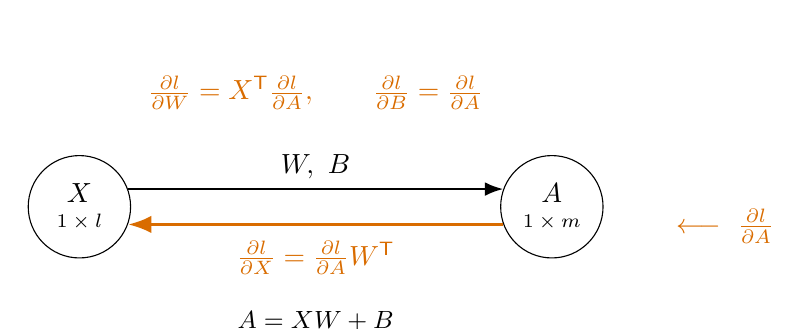
\begin{tikzpicture}[>=Latex]
\node[draw,circle,minimum size=13mm,align=center] (X) at (0,0) {$X$\\[-3pt]{\scriptsize $1\times l$}};
\node[draw,circle,minimum size=13mm,align=center] (A) at (6,0) {$A$\\[-3pt]{\scriptsize $1\times m$}};
\draw[->,thick] (X.20) -- node[above] {$W,\ B$} (A.160);
\draw[<-,very thick,orange!85!black] (X.-20) -- node[below=2pt] {$\pd{l}{X}=\pd{l}{A}W\T$} (A.-160);
\node[font=\small] at (3,-1.45) {$A=XW+B$};
\node[orange!85!black] at (8.2,-0.25) {$\longleftarrow\ \pd{l}{A}$};
\node[orange!85!black] at (3,1.45) {$\pd{l}{W}=X\T\pd{l}{A},\qquad \pd{l}{B}=\pd{l}{A}$};
\end{tikzpicture}

\small (1) 변수 노드 기준의 affine 계층
\end{minipage}
\end{center}

\begin{center}
\begin{minipage}{\textwidth}
\centering
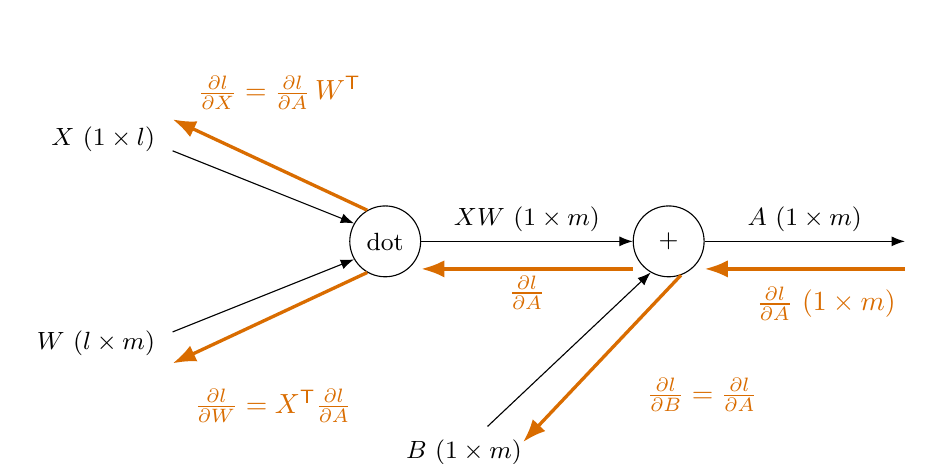
\begin{tikzpicture}[>=Latex,
  op/.style={draw,circle,minimum size=9mm,inner sep=0pt,font=\small},
  bw/.style={<-,very thick,orange!85!black},
  bl/.style={orange!85!black,font=\normalsize}]
\node[op] (dot) at (3,0.6) {dot};
\node[op] (pl) at (6.6,0.6) {$+$};
% forward
\node[font=\small,anchor=east] (X) at (0.2,1.9) {$X\ (1\times l)$};
\node[font=\small,anchor=east] (W) at (0.2,-0.7) {$W\ (l\times m)$};
\node[font=\small,anchor=north] (B) at (4.0,-1.8) {$B\ (1\times m)$};
\draw[->] (0.3,1.75) -- (dot.150);
\draw[->] (0.3,-0.55) -- (dot.210);
\draw[->] (dot.east) -- node[above,font=\small] {$XW\ (1\times m)$} (pl.west);
\draw[->] (4.3,-1.75) -- (pl.240);
\draw[->] (pl.east) -- node[above,font=\small] {$A\ (1\times m)$} (9.6,0.6);
% backward
\draw[bw] (0.3,2.15) -- (dot.120);
\draw[bw] (0.3,-0.95) -- (dot.240);
\draw[bw] ([yshift=-3.5mm]dot.east) -- ([yshift=-3.5mm]pl.west);
\draw[bw] (4.75,-1.95) -- (pl.290);
\draw[bw] ([yshift=-3.5mm]pl.east) -- ([yshift=-3.5mm]9.6,0.6);
\node[bl,anchor=south west] at (0.5,2.15) {$\pd{l}{X}=\pd{l}{A}\,W\T$};
\node[bl,anchor=north east] at (2.7,-1.15) {$\pd{l}{W}=X\T\pd{l}{A}$};
\node[bl,anchor=west] at (6.2,-1.35) {$\pd{l}{B}=\pd{l}{A}$};
\node[bl] at (4.8,-0.05) {$\pd{l}{A}$};
\node[bl,anchor=north] at (8.6,0.15) {$\pd{l}{A}\ (1\times m)$};
\end{tikzpicture}

\small (2) 연산 노드 기준의 affine 계층 (괄호 안은 shape)
\end{minipage}
\end{center}

연산 노드 기준의 그림에서는 역전파를 \textbf{연산 노드마다 하나의 규칙}으로 읽을 수 있다.
각 노드는 출력 쪽(upstream)에서 흘러 들어온 gradient를 받아, 입력 쪽(downstream) 변수들로 전달한다.
\begin{itemize}[leftmargin=1.8em]
\item \textbf{$+$ 노드} ($A=P+B$):
$\pd{A}{P}=\pd{A}{B}=1$이므로 upstream gradient를 \textbf{그대로} 두 입력에 전달한다.
\[
\pd{l}{P}=\pd{l}{A},\qquad \pd{l}{B}=\pd{l}{A}
\]
\item \textbf{dot 노드} ($P=XW$):
upstream gradient $\pd{l}{P}$에 \textbf{반대편 입력의 transpose}를 행렬곱하여 전달한다.
\[
\pd{l}{X}=\pd{l}{P}\,W\T,
\qquad
\pd{l}{W}=X\T\,\pd{l}{P}
\]
곱하는 위치는 순전파 $P=XW$에서 상대 행렬이 있던 쪽이며,
앞의 ``등식을 넘어가면 transpose''와 같은 규칙이다.
\end{itemize}


% =================================================
\section{활성화 계층의 역전파}
% =================================================

활성화 함수 $h$에 의하여
\[
Z=(z_1,\ldots,z_m)=h(A)=\bigl(h(a_1),\ldots,h(a_m)\bigr)
\]
로 연결되어 있다고 하자.
$Z$층까지의 역전파 $\pd{l}{Z}=\left(\pd{l}{z_1},\ldots,\pd{l}{z_m}\right)$를 알고 있을 때
$\pd{l}{A}$를 구하자.
$a_j$는 $z_j$에\textbf{만} 연결되므로 합은 필요 없고
\[
\pd{l}{a_j}=\pd{z_j}{a_j}\pd{l}{z_j}=h'(a_j)\pd{l}{z_j}
\]
이다. 즉 활성화 계층의 역전파는 \textbf{성분별 곱}이다.

\subsection{Sigmoid 활성화 함수}

$h(a)=\sigmoid(a)=\dfrac{1}{1+e^{-a}}$이면 $\pd{z}{a}=z(1-z)$이므로
\[
\pd{l}{A}
=\left(z_1(1-z_1)\pd{l}{z_1},\ldots,z_m(1-z_m)\pd{l}{z_m}\right)
=\boxed{Z\odot(1-Z)\odot\pd{l}{Z}}
\]
이다. 여기서 $\odot$는 성분끼리의 곱(아다마르 곱)이고, $1$은 $Z$와 같은 shape의 모든 성분이 $1$인 행렬이다.
NumPy에서는 \texttt{Z * (1 - Z) * dZ}처럼 \texttt{*}로 쓴다.

\begin{center}
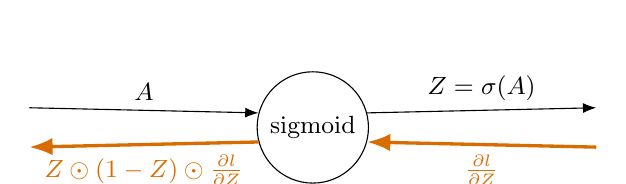
\begin{tikzpicture}[>=Latex]
\node[draw,circle,minimum size=13mm,font=\small] (s) at (0,0) {sigmoid};
\draw[->] (-3.6,0.25) -- node[above,font=\small] {$A$} (s.165);
\draw[->] (s.15) -- node[above,font=\small] {$Z=\sigmoid(A)$} (3.6,0.25);
\draw[<-,very thick,orange!85!black] (-3.6,-0.25) -- node[below,font=\small] {$Z\odot(1-Z)\odot\pd{l}{Z}$} (s.195);
\draw[<-,very thick,orange!85!black] (s.-15) -- node[below,font=\small] {$\pd{l}{Z}$} (3.6,-0.25);
\end{tikzpicture}

\small sigmoid 계층: 순전파의 출력 $Z$만 기억해 두면 역전파를 계산할 수 있다.
\end{center}

\subsection{ReLU 활성화 함수}

$h(a)=\max(0,a)=\begin{cases}a,&a>0\\0,&a\le0\end{cases}$이면
$h'(a)=\begin{cases}1,&a>0\\0,&a<0\end{cases}$이므로
\[
\pd{l}{a_j}=
\begin{cases}
\pd{l}{z_j},& a_j>0\\[4pt]
0,& a_j\le0
\end{cases}
\qquad\Longrightarrow\qquad
\boxed{\pd{l}{A}=\mathbf{1}[A>0]\odot\pd{l}{Z}}
\]
이다. 여기서 $\mathbf{1}[A>0]$은 \textbf{지시함수(indicator function)}로,
$a_j>0$인 성분은 $1$, 나머지는 $0$인 $A$와 같은 shape의 행렬이다
(계단함수를 써서 $\mathrm{step}(A)$로 쓰기도 한다).
꺾이는 점 $a_j=0$에서는 $h'(0)=0$으로 약속한다.
즉 ReLU는 입력이 양수였던 node의 기울기는 \textbf{그대로 통과}시키고,
입력이 $0$ 이하였던 node의 기울기는 \textbf{$0$으로 막는다}.
NumPy에서는 \texttt{np.where(A > 0, dZ, 0)}이다.

\begin{center}
\begin{tikzpicture}[>=Latex]
% a > 0
\begin{scope}
\node[draw,circle,minimum size=11mm,font=\small] (r) at (0,0) {ReLU};
\draw[->] (-2.8,0.25) -- node[above,font=\small] {$a_j$} (r.165);
\draw[->] (r.15) -- node[above,font=\small] {$z_j=a_j$} (2.8,0.25);
\draw[<-,very thick,orange!85!black] (-2.8,-0.25) -- node[below,font=\small] {$\pd{l}{z_j}$} (r.195);
\draw[<-,very thick,orange!85!black] (r.-15) -- node[below,font=\small] {$\pd{l}{z_j}$} (2.8,-0.25);
\node[font=\small] at (0,1.15) {$a_j>0$: 기울기를 그대로 통과};
\end{scope}
% a <= 0
\begin{scope}[xshift=7.4cm]
\node[draw,circle,minimum size=11mm,font=\small] (r) at (0,0) {ReLU};
\draw[->] (-2.8,0.25) -- node[above,font=\small] {$a_j$} (r.165);
\draw[->] (r.15) -- node[above,font=\small] {$z_j=0$} (2.8,0.25);
\draw[<-,very thick,orange!85!black] (-2.8,-0.25) -- node[below,font=\small] {$0$} (r.195);
\draw[<-,very thick,orange!85!black] (r.-15) -- node[below,font=\small] {$\pd{l}{z_j}$} (2.8,-0.25);
\node[font=\small] at (0,1.15) {$a_j\le0$: 기울기를 $0$으로 막음};
\end{scope}
\end{tikzpicture}

\small ReLU 계층: 순전파 때 $a_j>0$이었는지(\texttt{mask})만 기억해 두면 된다.
\end{center}


이렇게 계산된 $\pd{l}{A}$는 2절의 affine 계층으로 전달되어
$\pd{l}{W^{(1)}}$, $\pd{l}{B^{(1)}}$, $\pd{l}{X}$를 계산하는 데 쓰인다.

% =================================================
\section{Affine 계층의 역전파 (은닉층과 출력층 사이)}
% =================================================

$Z_{1\times m}$에서 $U=(u_1,\ldots,u_n)$로의 affine 변환
\[
U_{1\times n}=Z_{1\times m}W^{(2)}_{m\times n}+B^{(2)}_{1\times n}
\]
도 2절과 \textbf{똑같은} 계층이다. 따라서 $U$층까지의 역전파 $\pd{l}{U}$로부터
\[
\pd{l}{Z}=\pd{l}{U}\,{W^{(2)}}\T,
\qquad
\pd{l}{W^{(2)}}=Z\T\pd{l}{U},
\qquad
\pd{l}{B^{(2)}}=\pd{l}{U}
\]
를 계산할 수 있다.
$\pd{l}{Z}$는 3절의 활성화 계층으로 전달되고,
$\pd{l}{W^{(2)}}$, $\pd{l}{B^{(2)}}$는 경사하강법에 사용된다.
같은 계층을 반복해서 쌓기 때문에 한 번 유도한 규칙을 몇 번이고 다시 쓸 수 있다.
이것이 역전파 알고리즘을 \textbf{계층(layer) 단위}로 구현하는 이유이다.

남은 것은 마지막 $U\to Y\to l$ 부분, 즉 $\pd{l}{U}$이다.
그 전에 먼저 출력 $U$를 정답과 어떻게 비교할지부터 정해야 한다.

% =================================================
\section{출력층의 설계: 정답을 어떻게 나타내고 무엇과 비교할까?}\label{sec:onehot}
% =================================================

\subsection{출력층 설계의 두 가지 질문}

은닉층까지의 계산은 모두 정했다. 이제 network의 \textbf{마지막 층}을 설계할 차례이다.
학습이란 결국 ``network의 출력이 정답에 가까워지도록'' parameter를 바꾸는 일이므로,
출력층을 설계할 때는 다음 두 질문에 답해야 한다.

\begin{keybox}[출력층 설계의 핵심 질문]
\begin{enumerate}[label=\textbf{Q\arabic*.},leftmargin=2.6em]
\item network의 \textbf{출력}과 \textbf{정답}을 각각 어떤 형태로 나타내야 서로 비교할 수 있을까?
\item 출력과 정답의 차이를 어떤 \textbf{손실함수}로 잴까?
(그리고 그 손실의 gradient는 학습하기에 좋은 모양일까?)
\end{enumerate}
\end{keybox}

\subsection{회귀에서는 두 질문이 쉬웠다}

지난주의 회귀 문제를 떠올려 보자.
network의 출력 $\widehat y$는 실수 하나이고, 정답 $t$도 실수 하나였다.
둘은 처음부터 \textbf{같은 종류의 양}이므로 바로 뺄 수 있었고 (Q1),
그 차이를 제곱한 $l=(\widehat y-t)^2$을 손실로 쓰면 되었다 (Q2).
출력층에서는 마지막 affine 계층의 값을 그대로 출력하면 되었다 (항등함수).

그렇다면 정답이 ``숫자 $0\sim9$ 중 어느 것인가''라는 \textbf{class}일 때는 어떻게 해야 할까?

\subsection{첫 번째 시도: class 번호를 출력 하나로 맞힌다면?}

가장 쉬운 방법은 회귀처럼 출력 node를 하나만 두고,
class 번호 $0,1,\ldots,9$를 정답 값으로 삼아 제곱 오차로 학습하는 것이다.
실제로 지난주 실습에서는 class $0,1,2,3$을 이렇게 계단 모양 함수로 회귀하였다.
하지만 MNIST에서는 이 방법에 근본적인 문제가 있다.

\begin{itemize}[leftmargin=1.8em]
\item \textbf{class 번호에 없던 크기와 순서가 생긴다.}
출력 하나로 번호를 맞히면 ``$3$과 $4$는 가깝고 $3$과 $8$은 멀다''고 가정하는 셈이다.
그러나 손글씨 숫자에서 $3$은 모양이 비슷한 $8$과 더 헷갈리기 쉽다.
번호는 이름표일 뿐, 크기의 의미가 없다.
\item \textbf{애매한 입력에서 엉뚱한 답이 나온다.}
$3$인지 $8$인지 헷갈리는 이미지에 대해 network는 오차를 줄이려고 두 값의 중간인 $5.5$ 근처를 출력하게 되고,
이를 반올림하면 전혀 관계없는 $5$나 $6$이 된다.
\item \textbf{얼마나 확신하는지를 나타낼 수 없다.}
출력 $5.5$만으로는 ``$3$일 가능성 반, $8$일 가능성 반''이라는 정보를 표현할 수 없다.
\end{itemize}
지난주 실습이 잘 된 것은 class들이 $x$축 위에 \textbf{순서대로 놓이도록} 데이터를 만들었기 때문이다.
일반적인 분류 문제에서는 class 사이에 그런 순서가 없다.

\subsection{두 번째 아이디어: class마다 출력 node를 하나씩}

그래서 출력층에 \textbf{class의 개수만큼} node를 둔다.
출력 $U=(u_1,\ldots,u_n)$의 $k$번째 성분 $u_k$는 ``입력이 $k$번째 class일 가능성''을 나타내는 어떠한 \textbf{점수(score)}이길 바란다. 이왕이면 출력층으로 보고 입력된 이미지가 각각의 class에 속하는지와 그 "확률"을 출력해주면 더 좋겠다.
class들은 서로 대등한 별개의 node가 되므로 번호의 크기나 순서는 아무 의미가 없어지고,
여러 class에 동시에 점수를 줄 수 있어 애매함도 표현할 수 있다.

이제 Q1의 절반, 즉 \textbf{정답의 표현}을 정하자.
출력이 $n$개의 성분을 가진 벡터이므로, 정답도 $n$개의 성분을 가진 벡터로 나타내야 비교할 수 있다.

class가 $n$개인 다중분류 문제에서 $k$번째 class의 정답(label, target)을
$k$번째 원소만 $1$이고 나머지는 모두 $0$인 벡터로 나타내는 방법을
\textbf{one-hot encoding}이라 하고, 이러한 벡터를 \textbf{one-hot vector}라 한다.

\begin{center}
\begin{tabular}{@{}cc@{}}
\toprule
class (target) & one-hot vector $t=(t_1,\ldots,t_n)$ \\
\midrule
$1$ & $(1,0,0,\ldots,0,0)$ \\
$2$ & $(0,1,0,\ldots,0,0)$ \\
$3$ & $(0,0,1,\ldots,0,0)$ \\
$\vdots$ & $\vdots$ \\
$n-1$ & $(0,0,0,\ldots,1,0)$ \\
$n$ & $(0,0,0,\ldots,0,1)$ \\
\bottomrule
\end{tabular}
\end{center}

예를 들어 MNIST에서 정답이 숫자 $5$인 이미지의 target은 (class $0,1,\ldots,9$의 순서로)
\[
t=(0,0,0,0,0,1,0,0,0,0)
\]
이다. 모든 class가 서로 같은 거리에 있으므로 번호의 크기와 순서가 사라진다.

\subsection{One-hot vector는 확률분포이다. 그런데 $U$는?}

one-hot vector $t$의 성분은 모두 $0$ 이상 $1$ 이하이고 합이 $1$이다.
즉 $t$는 ``정답 class일 확률이 $1$, 나머지 class일 확률이 $0$''인 \textbf{확률분포}로 볼 수 있다.

그런데 network의 출력 $U$는 affine 계층의 결과이므로
각 성분이 음수일 수도, $1$보다 클 수도 있고, 합도 $1$이 아니다.
예를 들어 정답이 첫 번째 class일 때
\[
U=(2.0,\ 1.0,\ 0.1),\qquad t=(1,\ 0,\ 0)
\]
은 서로 다른 종류의 양이어서 그대로 비교하기 어렵다.
정답은 확률분포인데 출력은 점수이니, Q1의 나머지 절반인 \textbf{출력의 표현}이 아직 정해지지 않은 것이다.

\subsection{출력층 설계의 답}

이 고민의 결론은 다음과 같다.

\begin{keybox}[출력층 설계의 답: one-hot / softmax / cross entropy]
\begin{enumerate}[label=\textbf{A\arabic*.},leftmargin=2.6em]
\item \textbf{정답}은 one-hot vector $t$로 나타낸다 (확률분포).
\textbf{출력}은 점수 $U$를 \textbf{softmax 계층}으로 확률분포 $Y$로 바꾼다
(\ref{sec:softmax}절). 이제 $Y$와 $t$는 같은 종류의 대상이다.
\item 두 확률분포 $Y$와 $t$의 차이는 \textbf{cross entropy}로 잰다 (\ref{sec:ce}절).
게다가 이 선택은 역전파를 $\pd{l}{U}=Y-t$라는 아주 간단한 식으로 만들어 준다
(\ref{sec:smce}, \ref{sec:whyce}절).
\end{enumerate}
\[
U\ (\text{점수})\ \xrightarrow{\ \text{softmax}\ }\ Y\ (\text{확률분포})\ \xrightarrow{\ \text{cross entropy}\ }\ l
\ \longleftarrow\ t\ (\text{one-hot, 확률분포})
\]
\end{keybox}

회귀와 비교하면, 문제의 종류에 따라 출력층의 세 가지 선택이 함께 정해진다는 것을 알 수 있다.

\begin{center}
\begin{tabular}{@{}llll@{}}
\toprule
문제 & 출력의 표현 & 정답의 표현 & 손실함수 \\
\midrule
회귀 & 실수 (항등함수) & 실수 & 제곱 오차 \\
다중분류 & 확률분포 (softmax) & 확률분포 (one-hot) & cross entropy \\
\bottomrule
\end{tabular}
\end{center}

다음 절부터 softmax와 cross entropy를 차례로 살펴본다.

% =================================================
\section{Softmax 계층: 점수를 확률분포로}\label{sec:softmax}
% =================================================

\subsection{정의와 성질}

점수 $U=(u_1,\ldots,u_n)$를 확률분포로 바꾸기 위해 다음 함수를 사용한다.
변수 $Y=(y_1,\ldots,y_n)$가
\[
\boxed{
y_i=\frac{e^{u_i}}{\sum_{k=1}^{n}e^{u_k}}=\frac{e^{u_i}}{e^{u_1}+e^{u_2}+\cdots+e^{u_n}},
\qquad i=1,\ldots,n
}
\]
로 $U=(u_1,\ldots,u_n)$의 함수로 정의하자. 그러면 $Y$는 다음 세 가지 성질을 만족한다.
\begin{enumerate}[label=\arabic*)]
\item $u_i$의 크기 순서와 $y_i$의 크기 순서가 일치한다. 즉 $u_i<u_j$이면 $y_i<y_j$이다.
\item $0<y_i<1$이다.
\item $\displaystyle\sum_{i=1}^{n}y_i=1$이다.
\end{enumerate}
이렇게 정의된 $U$에서 $Y$로의 함수를 \textbf{softmax 함수}라 하고 $Y=\softmax(U)$로 표시한다.

성질 2), 3) 때문에 $y_k$를 입력 $X$가 \textbf{$k$번째 class에 속할 확률}로 해석할 수 있다.
즉 출력층 $U$의 각 원소가 $X$가 $k$번째 class에 속할 ``점수''라면,
softmax는 이 점수를 ``확률''로 바꾸어 주는 함수이다.
성질 1) 때문에 가장 큰 점수를 받은 class가 가장 큰 확률을 받는다.
이제 network의 출력 $Y$와 정답 $t$는 \textbf{둘 다 확률분포}이므로 서로 직접 비교할 수 있다. (두 확률 분포를 어떻게 비교할 수 있을까?)



\begin{center}
\begin{tikzpicture}[x=0.9cm,y=1.6cm]
% scores
\begin{scope}
\draw[->] (-0.3,0) -- (3.4,0);
\draw[->] (-0.3,0) -- (-0.3,2.4);
\foreach \i/\v/\c in {1/2.0/blue!60, 2/1.0/blue!45, 3/0.1/blue!30}
  { \fill[\c] (\i-0.35,0) rectangle (\i+0.35,\v);
    \node[above,font=\small] at (\i,\v) {$\v$};
    \node[below,font=\small] at (\i,0) {$u_{\i}$}; }
\node[font=\small] at (1.5,2.75) {점수 $U$};
\end{scope}
\draw[->,thick,orange!80!black] (3.9,1.1) -- node[above,font=\small] {softmax} (5.6,1.1);
% probabilities
\begin{scope}[xshift=5.4cm]
\draw[->] (-0.3,0) -- (3.4,0);
\draw[->] (-0.3,0) -- (-0.3,2.4);
\draw[gray!50,dashed] (-0.3,2) -- (3.4,2) node[right,font=\scriptsize,black] {$1$};
\foreach \i/\v/\p/\c in {1/1.318/0.659/orange!70, 2/0.485/0.242/orange!55, 3/0.197/0.099/orange!40}
  { \fill[\c] (\i-0.35,0) rectangle (\i+0.35,\v);
    \node[above,font=\small] at (\i,\v) {$\p$};
    \node[below,font=\small] at (\i,0) {$y_{\i}$}; }
\node[font=\small] at (1.5,2.75) {확률 $Y$ (합 $=1$)};
\end{scope}
\end{tikzpicture}
\end{center}



예를 들어 $U=(2.0,\ 1.0,\ 0.1)$이면 $e^{2}\approx7.389$, $e^{1}\approx2.718$, $e^{0.1}\approx1.105$이므로
\[
Y=\softmax(U)\approx\left(\frac{7.389}{11.213},\ \frac{2.718}{11.213},\ \frac{1.105}{11.213}\right)\approx(0.659,\ 0.242,\ 0.099)
\]
이다.

MNIST에서는 입력 이미지가 affine 계층과 ReLU 계층을 거쳐 10개 class의 점수 $U$가 되고,
softmax 계층이 이 점수를 합이 $1$인 확률 $Y$로 바꾼다.
아래 예에서 숫자 `2'의 점수 $6.0$은 확률 $0.928$ $(92.8\%)$로,
숫자 `0'의 점수 $1.0$은 확률 $0.006$으로 바뀐다.

\begin{center}
\begin{tikzpicture}[>=Latex,
  lay/.style={draw,rounded corners=2pt,minimum width=11mm,minimum height=30mm,font=\small,fill=softblue}]
\node[draw,minimum size=9mm,fill=black,text=white,font=\Large\bfseries] (img) at (0,0) {2};
\node[lay] (a1) at (1.8,0) {Affine};
\node[lay] (r1) at (3.3,0) {ReLU};
\node[lay] (a2) at (4.8,0) {Affine};
\node[lay,fill=orange!15] (sm) at (8.6,0) {Softmax};
\draw[->] (img) -- (a1); \draw[->] (a1) -- (r1); \draw[->] (r1) -- (a2);
% scores
\node[font=\small] at (6.7,1.95) {점수 $U$};
\foreach \y/\lbl/\v in {1.2/0/1.0, 0.6/1/-0.5, 0/2/6.0, -1.2/9/-0.2}
  { \draw[->] (a2.east |- 0,\y) -- (sm.west |- 0,\y);
    \node[font=\scriptsize,above] at (6.7,\y) {$u_{\lbl}=\v$}; }
\node at (6.7,-0.55) {$\vdots$};
% probabilities
\node[font=\small] at (10.6,1.95) {확률 $Y$};
\foreach \y/\lbl/\p in {1.2/0/0.006, 0.6/1/0.001, 0/2/0.928, -1.2/9/0.002}
  { \draw[->] (sm.east |- 0,\y) -- (11.6,\y);
    \node[font=\scriptsize,above] at (10.6,\y) {$y_{\lbl}=\p$}; }
\node at (10.6,-0.55) {$\vdots$};
\end{tikzpicture}
\end{center}

학습이 끝난 뒤 \textbf{예측(추론)}만 할 때는 가장 큰 점수의 class만 고르면 되므로 softmax를 생략해도 된다
(성질 1)). softmax는 \textbf{학습}할 때 손실을 계산하기 위해 필요하다.

\subsection{수치적으로 안전한 계산}

$e^{u}$는 $u$가 조금만 커져도 매우 커져서 컴퓨터에서 overflow가 일어난다
(예: $e^{1000}$).
그런데 임의의 상수 $c$에 대하여
\[
\frac{e^{u_i-c}}{\sum_k e^{u_k-c}}
=\frac{e^{-c}e^{u_i}}{e^{-c}\sum_k e^{u_k}}
=\frac{e^{u_i}}{\sum_k e^{u_k}}
\]
이므로 $\softmax(U-c)=\softmax(U)$이다.
따라서 $c=\max_k u_k$를 빼고 계산하면 지수의 최댓값이 $e^0=1$이 되어 안전하다.
\begin{lstlisting}
def softmax(U):
    U = U - np.max(U, axis=1, keepdims=True)   # same result, avoids overflow of exp
    expU = np.exp(U)
    return expU / np.sum(expU, axis=1, keepdims=True)
\end{lstlisting}
(\texttt{axis=1}은 한 데이터, 즉 한 \textbf{행} 안에서 $n$개 class에 대해 계산한다는 뜻이다.)

% =================================================
\section{Cross entropy 손실함수}\label{sec:ce}
% =================================================

이제 softmax 출력 $Y=(y_1,\ldots,y_n)$와 one-hot vector $t=(t_1,\ldots,t_n)$는 둘 다 확률분포이다.
이 두 확률분포의 차이로 손실함수를 정의하자.
제곱 손실
\[
l=\sum_{i=1}^{n}(y_i-t_i)^2
\]
을 사용할 수도 있으나, 다중분류 문제에서는 \textbf{cross entropy error}를 사용하는 것이 일반적이다:
\[
\boxed{
l=-\sum_{i=1}^{n}t_i\log y_i
}
\]
여기서 $\log$는 자연로그 $\ln$이다.
지금까지는 제곱 오차를 써 왔는데 왜 갑자기 cross entropy를 쓰는지는
먼저 그 의미와 역전파를 살펴본 뒤 \ref{sec:whyce}절에서 자세히 이야기한다.

$t$가 $k$번째 class를 나타내는 one-hot vector라면 $t_k$만 $1$이고 나머지는 모두 $0$이므로
실제로는 하나의 항만 남아
\[
l=-\log y_k
\]
이다. 즉 cross entropy는 \textbf{정답 class에 준 확률의 로그에 마이너스를 붙인 값}이다.

\begin{center}
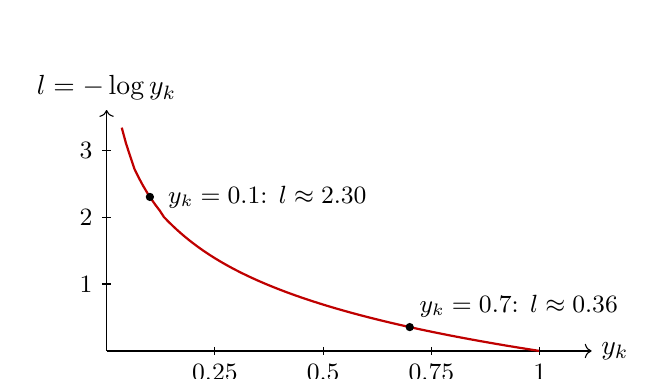
\begin{tikzpicture}[x=5.5cm,y=0.85cm]
\draw[->] (0,0) -- (1.12,0) node[right] {$y_k$};
\draw[->] (0,0) -- (0,3.6) node[above] {$l=-\log y_k$};
\draw[thick,red!75!black,domain=0.035:1,samples=100] plot (\x,{-ln(\x)});
\foreach \v in {0.25,0.5,0.75,1}
  \draw (\v,0.06) -- (\v,-0.06) node[below,font=\small] {$\v$};
\foreach \v in {1,2,3}
  \draw (0.01,\v) -- (-0.01,\v) node[left,font=\small] {$\v$};
\fill (0.7,{-ln(0.7)}) circle (1.5pt) node[above right,font=\small] {$y_k=0.7$: $l\approx0.36$};
\fill (0.1,{-ln(0.1)}) circle (1.5pt) node[right,font=\small] {$\ y_k=0.1$: $l\approx2.30$};
\end{tikzpicture}
\end{center}

$0<y_k<1$이므로 $l=-\log y_k>0$이고, $y_k\to1$일 때 $l\to0$, $y_k\to0$일 때 $l\to\infty$이다.
따라서 cross entropy 손실 $l$을 줄이도록 network를 훈련시킨다는 것은
\begin{itemize}[leftmargin=1.8em]
\item 정답 class의 node $y_k$의 값을 $1$에 가깝게 출력하도록 하고,
\item $Y$의 원소의 합이 $1$이므로 나머지 node는 $0$에 가깝게 출력하도록,
\end{itemize}
즉 $Y$가 one-hot vector $t$에 가까워지도록 훈련하는 것이다.
그러면 훈련된 network의 출력 $Y$를 보고 입력 $X$가 어떤 class에 속할 확률이 가장 큰지 판단할 수 있다.

예를 들어 정답이 $t=(0,1,0)$일 때
\[
Y=(0.1,\ 0.7,\ 0.2)\ \Rightarrow\ l=-\log0.7\approx0.36,
\qquad
Y=(0.6,\ 0.3,\ 0.1)\ \Rightarrow\ l=-\log0.3\approx1.20
\]
이다. 정답에 낮은 확률을 준 두 번째 경우를 훨씬 크게 벌한다.

\begin{remarkbox}[$\log 0$ 문제]
$y_k$가 $0$에 매우 가까우면 $\log y_k\to-\infty$가 되어 계산이 깨진다.
코드에서는 아주 작은 수를 더해 \texttt{np.log(Y + 1e-12)}로 계산한다.
\end{remarkbox}

% =================================================
\section{Softmax--cross entropy 계층의 역전파}\label{sec:smce}
% =================================================

이제 손실 $l$의 $u_i$에 대한 미분 $\pd{l}{u_i}$를 계산하자.
$u_i$는 softmax 때문에 $Y$층의 \textbf{모든} node $y_1,\ldots,y_n$을 거쳐 $l$에 연결되므로
\[
\pd{l}{u_i}=\sum_{j=1}^{n}\pd{y_j}{u_i}\pd{l}{y_j}
\]
이다.

\subsection{Softmax의 미분 $\partial y_j/\partial u_i$}

$S=e^{u_1}+\cdots+e^{u_n}$이라 하면 $y_j=e^{u_j}/S$이고 $\pd{S}{u_i}=e^{u_i}$이다.
몫의 미분법에 의해 두 가지 경우로 나뉜다.

\textbf{(1) $j=i$인 경우}
\[
\pd{y_i}{u_i}
=\frac{e^{u_i}\,S-e^{u_i}\,e^{u_i}}{S^2}
=\frac{e^{u_i}}{S}-\left(\frac{e^{u_i}}{S}\right)^2
=y_i-y_i^2=y_i(1-y_i)
\]

\textbf{(2) $j\ne i$인 경우} ($e^{u_j}$는 $u_i$에 대해 상수)
\[
\pd{y_j}{u_i}
=\frac{0\cdot S-e^{u_j}\,e^{u_i}}{S^2}
=-\frac{e^{u_j}}{S}\cdot\frac{e^{u_i}}{S}
=-y_jy_i
\]

\subsection{Cross entropy의 미분과 결합}

$l=-\sum_j t_j\log y_j$에서 로그함수의 미분법에 의해
\[
\pd{l}{y_j}=-\frac{t_j}{y_j}
\]
이다. 따라서 합성함수 미분법에 의해
\[
\begin{aligned}
\pd{l}{u_i}
&=\underbrace{y_i(1-y_i)\times\left(-\frac{t_i}{y_i}\right)}_{j=i}
+\sum_{j\ne i}\underbrace{(-y_jy_i)\times\left(-\frac{t_j}{y_j}\right)}_{j\ne i}\\
&=(y_i-1)\,t_i+\sum_{j\ne i}y_i\,t_j
=y_i\,(t_1+t_2+\cdots+t_n)-t_i\\
&=y_i-t_i
\end{aligned}
\]
이다. 여기서 one-hot vector는 $t_1+t_2+\cdots+t_n=1$이라는 사실을 이용하였다. 따라서

\begin{keybox}[Softmax--cross entropy 계층의 역전파]
\[
\boxed{
\pd{l}{U}=\left(\pd{l}{u_1},\ldots,\pd{l}{u_n}\right)=(y_1-t_1,\ldots,y_n-t_n)=Y-t
}
\]
softmax 계층과 cross entropy 손실을 하나로 묶으면,
역전파는 \textbf{예측 확률에서 정답을 뺀 값}이라는 매우 간단한 형태가 된다.
\end{keybox}

여기서 손실 $l$의 softmax 층에 대한 미분 $\pd{l}{Y}$를 따로 계산해 전달하지 않고,
softmax 층과 cross entropy 오차를 묶어서 ``softmax--cross entropy'' 층에 대한 역전파 $\pd{l}{U}$를
바로 나타냈음에 주목하자.
$\pd{l}{Y}=-t/Y$와 $n\times n$ Jacobian $\pd{Y}{U}$를 각각 계산해 곱하는 것보다
훨씬 간단하고 수치적으로도 안정적이다.
class가 3개인 경우의 계산 그래프로 나타내면 다음과 같다.

\begin{center}
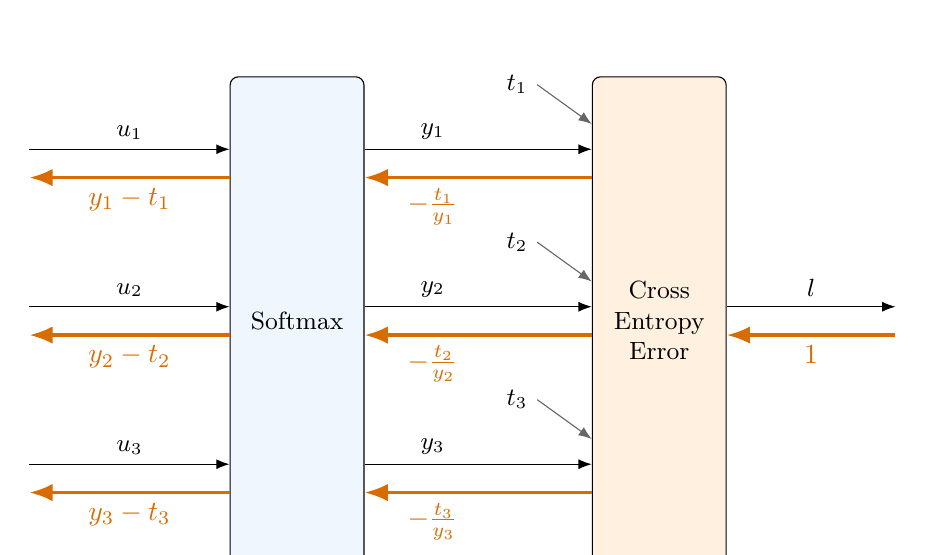
\begin{tikzpicture}[>=Latex,
  big/.style={draw,rounded corners=3pt,minimum width=17mm,minimum height=62mm,font=\small,align=center},
  bw/.style={<-,very thick,orange!85!black},
  bl/.style={orange!85!black,font=\normalsize}]
\node[big,fill=softblue] (sm) at (2.8,0) {Softmax};
\node[big,fill=orange!12] (ce) at (7.4,0) {Cross\\ Entropy\\ Error};
\foreach \y/\i in {2.0/1, 0/2, -2.0/3} {
  % input u_i
  \draw[->] (-0.6,\y+0.18) -- node[above,font=\small] {$u_{\i}$} (sm.west |- 0,\y+0.18);
  \draw[bw] (-0.6,\y-0.18) -- node[below,bl] {$y_{\i}-t_{\i}$} (sm.west |- 0,\y-0.18);
  % y_i
  \draw[->] (sm.east |- 0,\y+0.18) -- node[above,font=\small,pos=0.3] {$y_{\i}$} (ce.west |- 0,\y+0.18);
  \draw[bw] (sm.east |- 0,\y-0.18) -- node[below,bl,pos=0.3] {$-\frac{t_{\i}}{y_{\i}}$} (ce.west |- 0,\y-0.18);
  % t_i
  \draw[->,black!60] (5.85,\y+1.0) node[left,font=\small,black] {$t_{\i}$} -- (ce.west |- 0,\y+0.5);
}
\draw[->] (ce.east |- 0,0.18) -- node[above,font=\small] {$l$} (10.4,0.18);
\draw[bw] (ce.east |- 0,-0.18) -- node[below,bl] {$1$} (10.4,-0.18);
\end{tikzpicture}

\small Softmax-with-Loss 계층: 역전파는 출력의 끝 $\pd{l}{l}=1$에서 출발하여 $Y-t$가 된다.
\end{center}

중간의 $-\dfrac{t_i}{y_i}$와 softmax의 Jacobian이 곱해지면서 복잡한 항들이 모두 소거되고,
softmax 계층의 출력과 정답의 \textbf{차이} $y_i-t_i$만 앞 계층으로 전달된다.
예를 들어 정답이 $t=(0,1,0)$일 때
\begin{itemize}[leftmargin=1.8em]
\item network가 $Y=(0.3,\,0.2,\,0.5)$를 출력하면 (제대로 인식하지 못함)
$\pd{l}{U}=(0.3,\,-0.8,\,0.5)$라는 \textbf{큰} 기울기가 전달되어 많이 배우고,
\item $Y=(0.01,\,0.99,\,0)$을 출력하면 (거의 맞힘)
$\pd{l}{U}=(0.01,\,-0.01,\,0)$이라는 \textbf{작은} 기울기가 전달되어 조금만 배운다.
\end{itemize}

\begin{thinkbox}[$Y-t$의 의미]
정답 class $k$에 대해서는 $\pd{l}{u_k}=y_k-1<0$이므로 경사하강법은 점수 $u_k$를 \textbf{올리고},
나머지 class에 대해서는 $\pd{l}{u_j}=y_j>0$이므로 점수 $u_j$를 \textbf{내린다}.
그리고 그 크기는 ``얼마나 틀렸는가''에 비례한다.
지난주 MSE에서의 $\pd{l}{y}=2(y-t)$와 비슷한 모양이라는 점도 확인하자.
\end{thinkbox}

% =================================================
\section{왜 cross entropy를 쓰는가?}\label{sec:whyce}
% =================================================

지난주까지는 제곱 오차를 손실함수로 사용했다.
그런데 다중분류에서는 왜 cross entropy를 쓸까?
세 가지 이유가 있다.

\subsection{두 확률분포가 얼마나 다른지를 재는 척도이다}

\paragraph{질문: 두 확률분포는 얼마나 닮았는가?}
같은 표본공간 $\Omega=\{1,2,3\}$ 위의 이산확률분포 세 개를 생각하자.
(두 분포를 비교하려면 \textbf{같은 표본공간} 위에서 정의되어 있어야 한다.
분류 문제에서는 표본공간이 class의 집합 $\{1,\ldots,n\}$이다.)
\[
p=(0.5,\ 0.3,\ 0.2),
\qquad
q_A=(0.45,\ 0.35,\ 0.2),
\qquad
q_B=(0.1,\ 0.2,\ 0.7)
\]
$p$를 기준이 되는 분포(정답 분포)라 하고, $q_A$, $q_B$를 각각 $p$와 겹쳐 확률질량함수를 그려 보면 다음과 같다.

\begin{center}
\begin{tikzpicture}[x=1.25cm,y=4.6cm]
\foreach \pan/\sh/\qa/\qb/\qc/\nm in {A/0/0.45/0.35/0.2/A, B/7.6/0.1/0.2/0.7/B}{
\begin{scope}[xshift=\sh cm]
\draw[->] (0.3,0) -- (4.0,0) node[right,font=\small] {$i$};
\draw[->] (0.3,0) -- (0.3,0.85);
\foreach \v in {0.2,0.4,0.6} {
  \draw[gray!25] (0.3,\v) -- (3.8,\v);
  \node[left,font=\scriptsize] at (0.3,\v) {$\v$}; }
\foreach \i/\pv/\qv in {1/0.5/\qa, 2/0.3/\qb, 3/0.2/\qc} {
  \fill[blue!55] (\i-0.33,0) rectangle (\i-0.01,\pv);
  \fill[orange!75] (\i+0.01,0) rectangle (\i+0.33,\qv);
  \node[below,font=\small] at (\i,0) {$\i$};
}
\fill[blue!55] (1.0,0.92) rectangle (1.3,0.97); \node[right,font=\small] at (1.3,0.945) {$p$};
\fill[orange!75] (2.1,0.92) rectangle (2.4,0.97); \node[right,font=\small] at (2.4,0.945) {$q_\nm$};
\end{scope}}
\node[font=\small] at (2.15,-0.16) {(가) $p$와 $q_A$: 거의 같다};
\node[font=\small] at (8.25,-0.16) {(나) $p$와 $q_B$: 많이 다르다};
\end{tikzpicture}
\end{center}

그림으로 보면 $q_A$는 $p$와 거의 같고 $q_B$는 $p$와 많이 다르다.
그렇다면 ``두 분포가 얼마나 다른가''를 \textbf{하나의 수}로 나타내려면 어떻게 해야 할까?
softmax가 내놓는 분포 $Y$를 정답 분포 $t$에 가깝게 만드는 것이 학습의 목표이므로,
이 질문에 대한 답이 곧 손실함수가 된다.

가장 먼저 떠오르는 방법은 성분별 차이의 제곱합 $\sum_i(p_i-q_i)^2$이다.
이것도 하나의 척도이지만, 확률분포라는 특성을 쓰지 않고 $p$, $q$를 그냥 벡터로 본 것이다.
확률분포에 걸맞은 척도는 ``\textbf{놀라움(surprise)}''이라는 개념에서 출발한다.

\paragraph{놀라움과 entropy.}
확률이 $q_i$인 사건이 일어났을 때의 놀라움을
\[
-\log q_i
\]
로 재자. 확률이 $1$인 사건이 일어나면 놀라움은 $0$이고,
확률이 작은 사건일수록 놀라움이 크다 ($q_i\to0$이면 $-\log q_i\to\infty$).
결과가 실제로 분포 $p$를 따라 일어날 때, 평균 놀라움
\[
H(p)=-\sum_{i=1}^{n}p_i\log p_i
\]
를 $p$의 \textbf{entropy}라 한다. 분포 $p$ 자체가 가진 불확실성의 크기이다.

\paragraph{Cross entropy: 틀린 분포로 놀라움을 잴 때.}
그런데 결과는 실제로 $p$를 따라 일어나는데,
우리가 그 분포를 $q$라고 \textbf{믿고} 놀라움을 $-\log q_i$로 잰다면 평균 놀라움은
\[
H(p,q)=-\sum_{i=1}^{n}p_i\log q_i
\]
가 된다. 이것을 $p$에 대한 $q$의 \textbf{cross entropy}라 한다.
$q$가 실제로 자주 일어나는 결과($p_i$가 큰 $i$)에 작은 확률을 줄수록 큰 놀라움이 자주 생겨
$H(p,q)$가 커진다.

\paragraph{KL divergence: 틀린 믿음 때문에 추가된 놀라움.}
$q$가 $p$와 정확히 같으면 cross entropy는 entropy와 같아진다: $H(p,p)=H(p)$.
그 차이
\[
\boxed{
D_{\mathrm{KL}}(p\,\|\,q)=H(p,q)-H(p)=\sum_{i=1}^{n}p_i\log\frac{p_i}{q_i}
}
\]
를 \textbf{KL divergence}(Kullback--Leibler divergence)라 한다.
$p$ 대신 $q$를 믿었기 때문에 \textbf{추가로} 생긴 평균 놀라움이며,
\[
D_{\mathrm{KL}}(p\,\|\,q)\ge0,\qquad D_{\mathrm{KL}}(p\,\|\,q)=0\iff p=q
\]
이다. 즉 KL divergence는 두 분포가 다를수록 커지는, 두 확률분포의 차이를 재는 척도이다.

\begin{remarkbox}[$D_{\mathrm{KL}}(p\,\|\,q)\ge0$의 증명]
모든 $x>0$에 대하여 $\log x\le x-1$이고 등호는 $x=1$일 때만 성립한다. 따라서
\[
-D_{\mathrm{KL}}(p\,\|\,q)=\sum_{i}p_i\log\frac{q_i}{p_i}
\le\sum_{i}p_i\left(\frac{q_i}{p_i}-1\right)
=\sum_i q_i-\sum_i p_i=1-1=0
\]
이고, 등호는 모든 $i$에 대해 $q_i/p_i=1$, 즉 $p=q$일 때만 성립한다.
(합은 $p_i>0$인 $i$에 대해서만 한다.)
KL divergence는 $D_{\mathrm{KL}}(p\|q)\ne D_{\mathrm{KL}}(q\|p)$일 수 있으므로
엄밀한 의미의 거리는 아니지만, 두 분포의 차이를 재는 척도로 널리 쓰인다.
\end{remarkbox}

위의 예에서 실제로 계산해 보면 다음과 같다 ($H(p)\approx1.030$).

\begin{center}
\begin{tabular}{@{}lccc@{}}
\toprule
& cross entropy $H(p,q)$ & KL divergence $D_{\mathrm{KL}}(p\|q)$ & (참고) $\sum_i(p_i-q_i)^2$ \\
\midrule
$q_A=(0.45,\,0.35,\,0.2)$ & $1.036$ & $0.006$ & $0.005$ \\
$q_B=(0.1,\,0.2,\,0.7)$ & $1.706$ & $0.676$ & $0.420$ \\
\bottomrule
\end{tabular}
\end{center}

그림에서 본 직관대로 $q_B$가 $p$에서 훨씬 멀다.
$q_B$는 $p$에서 가장 자주 일어나는 결과 $1$ ($p_1=0.5$)에 확률 $0.1$만 주었으므로,
그 결과가 일어날 때마다 놀라움이 $-\log0.1\approx2.30$으로 크다.

\paragraph{정답 분포가 고정되어 있으면: KL을 줄이는 것 = cross entropy를 줄이는 것.}
위 식을 다시 쓰면
\[
H(p,q)=\underbrace{H(p)}_{p\text{만의 함수}}+D_{\mathrm{KL}}(p\,\|\,q)
\]
이다. 학습에서 $p$는 \textbf{정답 분포 $t$}로 \textbf{고정}되어 있고,
우리가 바꿀 수 있는 것은 network의 출력 분포 $q=Y=\softmax(U)$뿐이다.
$p$가 고정되면 entropy $H(p)$는 \textbf{상수}이므로,
\[
\text{KL divergence } D_{\mathrm{KL}}(t\,\|\,Y)\text{를 작게 하는 것}
\iff
\text{cross entropy } H(t,Y)\text{를 작게 하는 것}
\]
이다. 두 분포의 차이(KL divergence)를 줄이는 방법은 cross entropy를 줄이는 것뿐이며,
cross entropy가 가장 작아지는 것은 $Y=t$일 때이다.
그래서 cross entropy를 손실함수로 쓴다.

\paragraph{One-hot 정답이면.}
정답이 $k$번째 class인 one-hot vector $t$이면 $t_k=1$이고 나머지는 $0$이므로
$H(t)=-1\cdot\log1=0$이다 (단, $0\log0=0$으로 약속한다). 따라서
\[
l=H(t,Y)=D_{\mathrm{KL}}(t\,\|\,Y)=-\log y_k
\qquad(k:\ \text{정답 class})
\]
가 되어 cross entropy와 KL divergence가 정확히 같아진다.
두 분포를 비교하는 일반적인 척도가, one-hot 정답과 만나면
\textbf{정답 node의 확률 하나만 보는} \ref{sec:ce}절의 간단한 해석이 되는 것이다.

\begin{remarkbox}[최대가능도(maximum likelihood)의 관점]
$y_k$는 network가 정답 class에 준 확률이므로,
데이터 $N$개에 대한 평균 손실
$\frac1N\sum_{i}\bigl(-\log y^{(i)}_{k_i}\bigr)=-\frac1N\log\prod_{i}y^{(i)}_{k_i}$을 최소화하는 것은
network가 \textbf{훈련 데이터의 정답들을 모두 맞힐 확률} $\prod_i y^{(i)}_{k_i}$을 최대화하는 것과 같다.
통계학에서 말하는 최대가능도 추정이다.
\end{remarkbox}

\subsection{Softmax와 짝을 이루어 역전파가 간단해진다}

\ref{sec:smce}절에서 보았듯이 softmax와 cross entropy를 묶으면
\[
\pd{l}{U}=Y-t
\]
라는 매우 간단한 역전파를 얻는다. 이것은 우연이 아니다.
지난주의 회귀 문제에서 출력층이 항등함수 $y=u$이고 손실이 제곱 오차일 때에도
$\pd{l}{u}=2(y-t)$로 ``출력 $-$ 정답'' 꼴이었다.
\begin{center}
\begin{tabular}{@{}lll@{}}
\toprule
문제 & 출력층 & 손실함수 \\
\midrule
회귀 & 항등함수 & 제곱 오차 \\
다중분류 & softmax & cross entropy \\
\bottomrule
\end{tabular}
\end{center}
이처럼 출력층의 함수와 손실함수를 \textbf{짝}으로 고르면
역전파가 ``출력과 정답의 차이''로 깔끔하게 떨어진다.

\subsection{제곱 오차로도 학습할 수 있을까?}

물론 가능하다. softmax 출력에 제곱 오차 $l=\frac12\sum_i(y_i-t_i)^2$를 쓰더라도
합성함수 미분법으로 역전파를 계산할 수 있다.
$\pd{l}{y_j}=y_j-t_j$와 softmax의 미분($\pd{y_j}{u_i}$, \ref{sec:smce}절)을 결합하면
\[
\pd{l}{u_i}
=\sum_{j=1}^{n}\pd{y_j}{u_i}\,(y_j-t_j)
=y_i\Bigl((y_i-t_i)-\sum_{j=1}^{n}y_j(y_j-t_j)\Bigr)
\]
이다 (연습문제 8). 실습 코드의 \texttt{SoftmaxWithSquaredError} 계층이 이 식을 구현한 것이며,
기울기 검사도 통과한다.
그러나 cross entropy와 비교하면 다음과 같은 약점이 있다.

\begin{itemize}[leftmargin=1.8em]
\item \textbf{확신을 갖고 틀리면 거의 배우지 못한다.}
위 식에는 $y_i$가 곱해져 있어서, 정답 class의 확률 $y_k$가 $0$에 가까우면 기울기도 $0$에 가까워진다.
예를 들어 $t=(1,0)$인데 network가 $Y=(0.01,\,0.99)$를 출력하면
\[
\text{cross entropy: }\pd{l}{U}=(-0.99,\ 0.99),
\qquad
\text{제곱 오차: }\pd{l}{U}\approx(-0.0196,\ 0.0196)
\]
로, 가장 많이 배워야 할 순간에 제곱 오차의 기울기는 \textbf{약 50배 작다}.
\item \textbf{학습 초기가 느리다.}
초기에는 모든 class의 확률이 $y_i\approx\frac1n$로 비슷하므로,
$y_i$가 곱해진 제곱 오차의 기울기는 작다.
\end{itemize}

실제로 scikit-learn에 들어 있는 $8\times8$ 손글씨 숫자 데이터(훈련 1500개, test 297개)로
같은 network(은닉 node 50개, 미니배치 50, 학습률 0.5)를 학습시키면 test 정확도는 다음과 같다.

\begin{center}
\begin{tabular}{@{}lcccc@{}}
\toprule
손실함수 & 5 epoch & 10 epoch & 20 epoch & 30 epoch \\
\midrule
softmax + cross entropy & 91.6\% & 96.3\% & 97.3\% & 97.6\% \\
softmax + 제곱 오차 & 22.6\% & 25.6\% & 91.6\% & 94.6\% \\
\bottomrule
\end{tabular}
\end{center}

제곱 오차도 결국 학습은 되지만 처음 10 epoch 동안 거의 진전이 없고, 최종 정확도도 낮다.

\begin{keybox}[다중분류에서 cross entropy를 쓰는 이유]
\begin{enumerate}[leftmargin=1.8em]
\item 정답 분포 $t$와 출력 분포 $Y$라는 \textbf{두 확률분포의 차이를 재는 척도}이며,
one-hot 정답이면 $-\log y_k$로 간단해진다.
\item softmax와 짝을 이루어 역전파가 $\pd{l}{U}=Y-t$로 \textbf{간단명료}해진다.
\item 틀린 정도에 비례하는 기울기를 주므로 제곱 오차보다 \textbf{빠르고 안정적으로} 학습한다.
\end{enumerate}
\end{keybox}

% =================================================
\section{정리: 데이터 하나에 대한 순전파와 역전파}\label{sec:summary}
% =================================================

가중치와 편이를 초기화한 상태에서 하나의 데이터 $X$와 정답 $t$에 대하여

\begin{keybox}[순전파와 역전파 한눈에 보기]
\textbf{순전파}
\[
A=XW^{(1)}+B^{(1)},
\ \
Z=h(A),
\ \
U=ZW^{(2)}+B^{(2)},
\ \
Y=\softmax(U),
\ \
l=-\sum_{i=1}^{n}t_i\log y_i
\]
\textbf{역전파} (순서를 거꾸로)
\[
\begin{aligned}
&\pd{l}{U}=Y-t\\[4pt]
&\pd{l}{W^{(2)}}=Z\T\pd{l}{U},
\qquad
\pd{l}{B^{(2)}}=\pd{l}{U},
\qquad
\pd{l}{Z}=\pd{l}{U}{W^{(2)}}\T\\[4pt]
&\pd{l}{A}=Z\odot(1-Z)\odot\pd{l}{Z}\ \ (\text{sigmoid})
\quad\text{또는}\quad
\pd{l}{A}=\mathbf{1}[A>0]\odot\pd{l}{Z}\ \ (\text{ReLU})\\[4pt]
&\pd{l}{W^{(1)}}=X\T\pd{l}{A},
\qquad
\pd{l}{B^{(1)}}=\pd{l}{A},
\qquad
\pd{l}{X}=\pd{l}{A}{W^{(1)}}\T
\end{aligned}
\]
\end{keybox}

이전 층까지의 역전파 결과가 다음 층의 역전파 계산에 그대로 쓰인다는 점에 주목하자.
이제 경사하강법으로 가중치와 편이를 갱신하면 된다.

\begin{center}
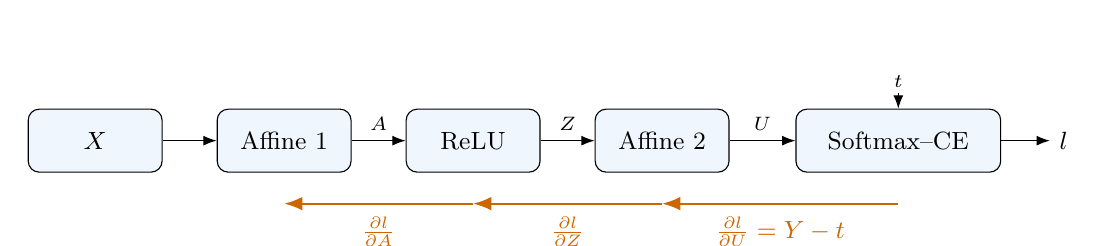
\begin{tikzpicture}[>=Latex,
  box/.style={draw,rounded corners,minimum width=17mm,minimum height=8mm,font=\small,fill=softblue}]
\node[box] (x) at (0,0) {$X$};
\node[box] (af1) at (2.4,0) {Affine 1};
\node[box] (act) at (4.8,0) {ReLU};
\node[box] (af2) at (7.2,0) {Affine 2};
\node[box,minimum width=26mm] (sm) at (10.2,0) {Softmax--CE};
\node[font=\small] (l) at (12.3,0) {$l$};
\draw[->] (x) -- (af1); \draw[->] (af1) -- node[above,font=\scriptsize] {$A$} (act);
\draw[->] (act) -- node[above,font=\scriptsize] {$Z$} (af2);
\draw[->] (af2) -- node[above,font=\scriptsize] {$U$} (sm); \draw[->] (sm) -- (l);
\node[font=\scriptsize] at (10.2,0.75) {$t$};
\draw[->] (10.2,0.6) -- (sm.north);
\draw[<-,thick,orange!80!black] ([yshift=-8mm]af1.center) -- node[below=1pt,font=\small] {$\pd{l}{A}$} ([yshift=-8mm]act.center);
\draw[<-,thick,orange!80!black] ([yshift=-8mm]act.center) -- node[below=1pt,font=\small] {$\pd{l}{Z}$} ([yshift=-8mm]af2.center);
\draw[<-,thick,orange!80!black] ([yshift=-8mm]af2.center) -- node[below=1pt,font=\small] {$\pd{l}{U}=Y-t$} ([yshift=-8mm]sm.center);
\end{tikzpicture}
\end{center}

% =================================================
\section{미니배치 학습}\label{sec:minibatch}
% =================================================

\subsection{온라인 학습, full-batch 학습, 미니배치 학습}

지금까지 유도한 역전파는 \textbf{데이터 하나}에 대한 것이었다.
그런데 훈련 데이터는 $N$개(MNIST에서는 $60000$개)이다.
가중치를 한 번 업데이트할 때 \textbf{몇 개의 데이터}를 보고 gradient를 계산할지에 따라
학습 방법을 세 가지로 나눌 수 있다.
한 번에 사용하는 데이터의 개수를 $h$라 하고,
그 $h$개에 대한 손실의 평균을
\[
L=\frac1h\sum_{k=1}^{h}l_k,
\qquad
\pd{L}{W}=\frac1h\sum_{k=1}^{h}\pd{l_k}{W},
\qquad
\pd{L}{B}=\frac1h\sum_{k=1}^{h}\pd{l_k}{B}
\]
라 하면, 업데이트는 모두 $W\leftarrow W-\alpha\pd{L}{W}$, $B\leftarrow B-\alpha\pd{L}{B}$의 꼴이다.

\begin{enumerate}[leftmargin=1.8em]
\item \textbf{온라인 학습} (stochastic gradient descent, $h=1$):
데이터를 \textbf{하나씩} 보고 그때마다 가중치를 업데이트한다.
과제 1처럼 손으로 계산할 때의 방식이다.
\item \textbf{Full-batch 학습} ($h=N$):
\textbf{전체} 데이터의 평균 gradient를 계산한 뒤 가중치를 한 번 업데이트한다.
지난주 실습에서 데이터 12개를 한꺼번에 흘려보낸 방식이다.
\item \textbf{미니배치 학습} ($1<h<N$):
전체 데이터에서 무작위로 고른 \textbf{작은 묶음}(미니배치) $h$개의 평균 gradient로 업데이트한다.
보통 $h=32\sim256$ 정도를 사용한다.
\end{enumerate}

\begin{center}
\begin{tabular}{@{}p{0.17\textwidth}p{0.37\textwidth}p{0.37\textwidth}@{}}
\toprule
방법 & 장점 & 단점 \\
\midrule
온라인 ($h=1$)
& 데이터 하나만 보면 바로 업데이트할 수 있어 업데이트가 자주 일어나고, 메모리가 적게 든다.
& gradient가 데이터 하나에 크게 좌우되어 \textbf{들쭉날쭉}하다.
데이터를 하나씩 처리하므로 행렬 연산의 병렬성을 살리지 못해 \textbf{느리다}. \\[3pt]
Full-batch ($h=N$)
& 전체 데이터의 정확한 평균 gradient를 쓰므로 업데이트 방향이 \textbf{안정적}이다.
& 업데이트 \textbf{한 번}에 $N$개를 모두 계산해야 한다.
$N$이 크면 한 걸음이 너무 느리고, 전체 데이터가 메모리에 들어가지 않을 수도 있다. \\[3pt]
미니배치 ($1<h<N$)
& 전체 평균의 \textbf{적당히 좋은 근사}를 \textbf{싸게} 얻는다.
$h$개를 행렬 한 번으로 계산하므로 빠르고, 1 epoch에 여러 번($N/h$번) 업데이트한다.
& gradient에 약간의 무작위성(잡음)이 남는다.
$h$라는 hyper-parameter를 정해야 한다. \\
\bottomrule
\end{tabular}
\end{center}

\begin{keybox}[왜 미니배치 학습을 주로 쓰는가?]
\begin{itemize}[leftmargin=1.8em]
\item 전체 데이터의 평균 gradient는 일부 데이터의 평균으로도 꽤 잘 근사된다.
$100$개로 계산한 방향과 $60000$개로 계산한 방향이 크게 다르지 않다면,
$60000$개를 다 계산해서 한 걸음 가는 것보다 $100$개씩 보고 $600$걸음 가는 편이 훨씬 빨리 내려간다.
\item 데이터 $h$개를 \textbf{행렬 한 번}으로 처리하므로,
데이터를 하나씩 처리하는 온라인 학습보다 같은 양의 데이터를 훨씬 빠르게 계산한다 (다음 절).
\item gradient에 남는 약간의 잡음은 오히려 학습에 도움이 되기도 한다.
\end{itemize}
즉 미니배치 학습은 full-batch의 \textbf{안정성}과 온라인 학습의 \textbf{잦은 업데이트} 사이의 절충이며,
현대 딥러닝은 거의 모두 미니배치 학습을 사용한다.
\end{keybox}

\subsection{행렬 연산으로 여러 데이터를 한꺼번에 순전파}

$h$개의 데이터 $X_1,\ldots,X_h$ (각각 $1\times l$)와 그 출력 $Y_k=X_kW+B$ (각각 $1\times m$)를
행으로 쌓아
\[
X=
\begin{bmatrix}
x_{11}&x_{12}&\cdots&x_{1l}\\
x_{21}&x_{22}&\cdots&x_{2l}\\
\vdots&&&\vdots\\
x_{h1}&x_{h2}&\cdots&x_{hl}
\end{bmatrix}_{h\times l}
\quad(\text{미니배치 데이터}),
\]
\[
Y=
\begin{bmatrix}
y_{11}&\cdots&y_{1m}\\
\vdots&&\vdots\\
y_{h1}&\cdots&y_{hm}
\end{bmatrix}_{h\times m}
\quad(\text{미니배치의 출력})
\]
이라 하면, 행렬 연산으로
\[
\boxed{
Y_{h\times m}=X_{h\times l}\,W_{l\times m}+B_{h\times m},
\qquad
B_{h\times m}=
\begin{bmatrix}
b_1&b_2&\cdots&b_m\\
\vdots&&&\vdots\\
b_1&b_2&\cdots&b_m
\end{bmatrix}
}
\]
으로 여러 데이터를 한꺼번에 순전파할 수 있다.
$B$는 같은 행 $(b_1,\ldots,b_m)$을 $h$번 복사한 것이며,
NumPy에서는 $1\times m$ 배열 \texttt{B}를 더하면 \textbf{broadcasting}으로 자동으로 행 방향으로 복사된다.

\subsection{왜 행렬 연산으로 한꺼번에 계산하는가? --- 병렬 연산과 GPU}

$Y=XW+B$를 데이터 하나씩, 성분 하나씩 계산하면
\[
y_{kj}=\sum_{i=1}^{l}x_{ki}w_{ij}+b_j
\qquad(k=1,\ldots,h,\ \ j=1,\ldots,m)
\]
을 $h\times m$번 반복해야 한다.
그런데 이 $h\times m$개의 값은 \textbf{서로 독립적}이다. $y_{11}$을 계산하는 데 $y_{23}$이 필요하지 않다.
따라서 여러 개를 \textbf{동시에(병렬로)} 계산할 수 있다.
행렬곱 $XW$ 한 번은 바로 이런 독립적인 곱셈과 덧셈을 한꺼번에 모아 놓은 것이다.

\begin{itemize}[leftmargin=1.8em]
\item \textbf{NumPy}: \texttt{X @ W}는 Python의 for loop가 아니라,
CPU에서 행렬 연산에 최적화된 수치 계산 라이브러리(BLAS)를 호출하여
여러 연산을 동시에(CPU의 여러 core와 벡터 연산 명령) 처리한다.
이렇게 반복문을 행렬 연산으로 바꾸는 것을 \textbf{벡터화(vectorization)}라 한다.
\item \textbf{GPU}: 원래 화면의 수많은 픽셀을 동시에 계산하기 위해 만들어진 장치로,
CPU보다 훨씬 많은 수천 개의 단순한 연산 장치를 가지고 있어
\textbf{같은 종류의 독립적인 계산을 대량으로 동시에} 하는 데 특화되어 있다.
신경망의 학습은 대부분 큰 행렬곱이므로 GPU에서 매우 빨라진다.
딥러닝에 GPU가 필요한 이유이다.
\item \textbf{PyTorch의 \texttt{torch.tensor}}: NumPy 배열과 비슷한 다차원 배열이지만,
\texttt{.to("cuda")}로 GPU에 올리면 \texttt{X @ W} 같은 연산을 GPU에서 병렬로 실행한다.
(여기에 역전파를 자동으로 계산하는 autograd 기능이 더해진다.)
\end{itemize}

\begin{remarkbox}[직접 확인해 보기: \texttt{loop\_vs\_matmul.py}]
데이터 $h=100$개, $l=784$, $m=100$인 affine 계층의 순전파를
(1) Python의 3중 for loop로, (2) \texttt{X @ W + B} 한 줄로 계산하여 시간을 비교한다.
\begin{lstlisting}
def forward_loop(X, W, B):
    A = np.zeros((X.shape[0], W.shape[1]))
    for k in range(X.shape[0]):            # one sample at a time
        for j in range(W.shape[1]):        # one output node at a time
            s = 0.0
            for i in range(X.shape[1]):    # a_kj = sum_i x_ki w_ij + b_j
                s += X[k, i] * W[i, j]
            A[k, j] = s + B[0, j]
    return A

def forward_matmul(X, W, B):
    return X @ W + B                       # all samples, all nodes at once
\end{lstlisting}
두 결과는 같지만, 강의 준비에 사용한 노트북 PC에서는
for loop가 약 $1.8$초, \texttt{X @ W + B}가 약 $0.3$ms로 \textbf{수천 배} 차이가 났다
(정확한 값은 컴퓨터마다 다르다).
미니배치를 행렬로 쌓아 한꺼번에 계산하는 이유가 여기에 있다.
\end{remarkbox}

이렇게 행렬 연산이 빠르기 때문에 데이터 $h$개를 처리하는 시간은
데이터 $1$개를 처리하는 시간의 $h$배보다 훨씬 적게 든다.
미니배치 크기 $h$를 너무 작게 잡으면 이 병렬성을 살리지 못하고,
너무 크게 잡으면 업데이트 횟수가 줄고 메모리가 부족해진다.
GPU를 쓸 때 미니배치 크기를 $32$, $64$, $128$, $256$ 정도로 잡는 것은 이런 절충의 결과이다.

\subsection{미니배치에 대한 역전파}

데이터 $X_k$를 순전파했을 때의 손실을 $l_k$라 하고, 평균 손실을 $L=\frac1h\sum_k l_k$라 하자.
\[
\pd{L}{X}:=
\begin{bmatrix}
\pd{L}{X_1}\\ \vdots\\ \pd{L}{X_h}
\end{bmatrix}_{h\times l},
\qquad
\pd{L}{Y}:=
\begin{bmatrix}
\pd{L}{Y_1}\\ \vdots\\ \pd{L}{Y_h}
\end{bmatrix}_{h\times m}
=\frac1h
\begin{bmatrix}
\pd{l_1}{Y_1}\\ \vdots\\ \pd{l_h}{Y_h}
\end{bmatrix}
\]
로 정의하자 ($k$번째 행이 $k$번째 데이터에 대한 기울기).
데이터 하나에 대한 결과 $\pd{l_k}{W}=X_k\T\pd{l_k}{Y_k}$ (2절)를 이용하면
\[
\begin{aligned}
\pd{L}{W}
&=\frac1h\left(X_1\T\pd{l_1}{Y_1}+\cdots+X_h\T\pd{l_h}{Y_h}\right)
=\frac1h
\begin{bmatrix}
x_{11}\pd{l_1}{y_{11}}+\cdots+x_{h1}\pd{l_h}{y_{h1}} & \cdots\\
\vdots&\ddots
\end{bmatrix}\\
&=
\begin{bmatrix}
x_{11}&x_{21}&\cdots&x_{h1}\\
\vdots&&&\vdots\\
x_{1l}&x_{2l}&\cdots&x_{hl}
\end{bmatrix}
\cdot\frac1h
\begin{bmatrix}
\pd{l_1}{y_{11}}&\cdots&\pd{l_1}{y_{1m}}\\
\vdots&&\vdots\\
\pd{l_h}{y_{h1}}&\cdots&\pd{l_h}{y_{hm}}
\end{bmatrix}
=X\T\pd{L}{Y}
\end{aligned}
\]
이다. 즉 $h$개의 \textbf{외적의 합}이 행렬곱 $X\T\pd{L}{Y}$ 한 번으로 계산된다.
마찬가지로
\[
\pd{L}{B}=\frac1h\sum_{k=1}^{h}\pd{l_k}{Y_k}
=\texttt{np.sum}\left(\pd{L}{Y},\ \texttt{axis=0}\right),
\qquad
\pd{L}{X}=
\begin{bmatrix}
\pd{L}{Y_1}W\T\\ \vdots\\ \pd{L}{Y_h}W\T
\end{bmatrix}
=\pd{L}{Y}W\T
\]
이다. $\pd{L}{B}$는 $\pd{L}{Y}$의 $h$개 행을 \textbf{세로 방향으로 더한} $1\times m$ 행렬이다.

\begin{keybox}[미니배치 affine 계층의 역전파]
순전파 $Y_{h\times m}=X_{h\times l}W_{l\times m}+B_{1\times m}$ ($B$는 broadcast)에 대하여
\[
\begin{aligned}
\left(\pd{L}{X}\right)_{h\times l}&=\left(\pd{L}{Y}\right)_{h\times m}\left(W\T\right)_{m\times l},
\qquad
\left(\pd{L}{W}\right)_{l\times m}=\left(X\T\right)_{l\times h}\left(\pd{L}{Y}\right)_{h\times m},\\[4pt]
\left(\pd{L}{B}\right)_{1\times m}&=\texttt{np.sum}\Bigl(\pd{L}{Y},\,\texttt{axis=0}\Bigr)
\end{aligned}
\]

\begin{center}
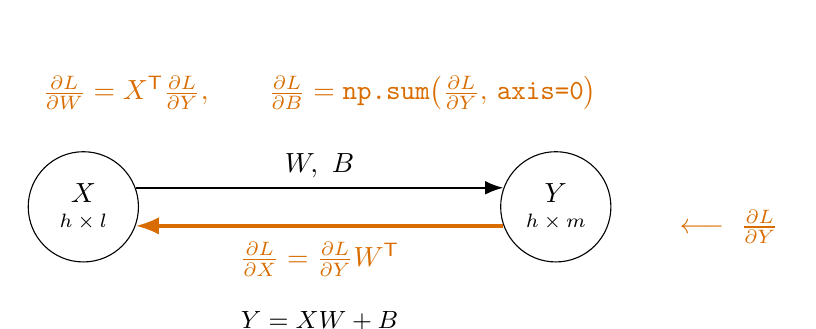
\begin{tikzpicture}[>=Latex]
\node[draw,circle,minimum size=14mm,align=center] (X) at (0,0) {$X$\\[-3pt]{\scriptsize $h\times l$}};
\node[draw,circle,minimum size=14mm,align=center] (Y) at (6,0) {$Y$\\[-3pt]{\scriptsize $h\times m$}};
\draw[->,thick] (X.20) -- node[above] {$W,\ B$} (Y.160);
\draw[<-,very thick,orange!85!black] (X.-20) -- node[below=2pt] {$\pd{L}{X}=\pd{L}{Y}W\T$} (Y.-160);
\node[font=\small] at (3,-1.45) {$Y=XW+B$};
\node[orange!85!black] at (8.2,-0.25) {$\longleftarrow\ \pd{L}{Y}$};
\node[orange!85!black] at (3,1.45) {$\pd{L}{W}=X\T\pd{L}{Y},\qquad \pd{L}{B}=\texttt{np.sum}\bigl(\pd{L}{Y},\,\texttt{axis=0}\bigr)$};
\end{tikzpicture}

\small (1) 변수 노드 기준
\end{center}

\begin{center}
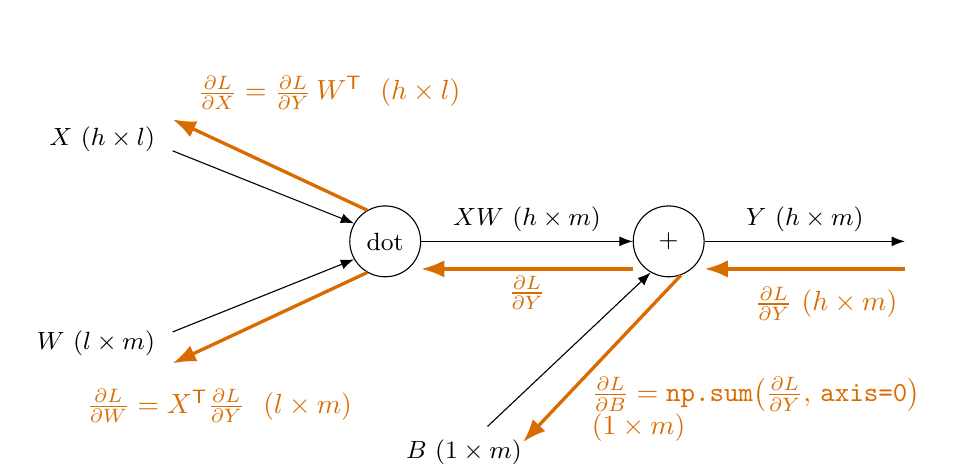
\begin{tikzpicture}[>=Latex,
  op/.style={draw,circle,minimum size=9mm,inner sep=0pt,font=\small},
  bw/.style={<-,very thick,orange!85!black},
  bl/.style={orange!85!black,font=\normalsize}]
\node[op] (dot) at (3,0.6) {dot};
\node[op] (pl) at (6.6,0.6) {$+$};
\node[font=\small,anchor=east] at (0.2,1.9) {$X\ (h\times l)$};
\node[font=\small,anchor=east] at (0.2,-0.7) {$W\ (l\times m)$};
\node[font=\small,anchor=north] at (4.0,-1.8) {$B\ (1\times m)$};
\draw[->] (0.3,1.75) -- (dot.150);
\draw[->] (0.3,-0.55) -- (dot.210);
\draw[->] (dot.east) -- node[above,font=\small] {$XW\ (h\times m)$} (pl.west);
\draw[->] (4.3,-1.75) -- (pl.240);
\draw[->] (pl.east) -- node[above,font=\small] {$Y\ (h\times m)$} (9.6,0.6);
\draw[bw] (0.3,2.15) -- (dot.120);
\draw[bw] (0.3,-0.95) -- (dot.240);
\draw[bw] ([yshift=-3.5mm]dot.east) -- ([yshift=-3.5mm]pl.west);
\draw[bw] (4.75,-1.95) -- (pl.290);
\draw[bw] ([yshift=-3.5mm]pl.east) -- ([yshift=-3.5mm]9.6,0.6);
\node[bl,anchor=south west] at (0.5,2.15) {$\pd{L}{X}=\pd{L}{Y}\,W\T\ \ (h\times l)$};
\node[bl,anchor=north east] at (2.7,-1.15) {$\pd{L}{W}=X\T\pd{L}{Y}\ \ (l\times m)$};
\node[bl,anchor=north west,align=left] at (5.5,-1.0) {$\pd{L}{B}=\texttt{np.sum}\bigl(\pd{L}{Y},\,\texttt{axis=0}\bigr)$\\ $(1\times m)$};
\node[bl] at (4.8,-0.05) {$\pd{L}{Y}$};
\node[bl,anchor=north] at (8.6,0.15) {$\pd{L}{Y}\ (h\times m)$};
\end{tikzpicture}

\small (2) 연산 노드 기준
\end{center}
데이터 하나일 때와 \textbf{같은 식}이며, $B$의 기울기만 $h$개 행을 더한다.
parameter의 업데이트도 같다:
\[
W\leftarrow W-\alpha\,X\T\pd{L}{Y},
\qquad
B\leftarrow B-\alpha\,\texttt{np.sum}\Bigl(\pd{L}{Y},\ \texttt{axis=0}\Bigr).
\]
\end{keybox}

\begin{remarkbox}[\texttt{axis=0}과 \texttt{axis=1}]
\texttt{np.sum(M, axis=0)}은 행렬 $M$의 \textbf{행들을 더한다} (세로 방향, 결과는 열마다 하나).
\texttt{np.sum(M, axis=1)}은 각 행 \textbf{안의 원소들을 더한다} (가로 방향, 결과는 행마다 하나).
미니배치에서는 행이 데이터이므로, 데이터에 대한 합은 \texttt{axis=0},
한 데이터 안의 class에 대한 합(softmax의 분모)은 \texttt{axis=1}이다.
\end{remarkbox}

\begin{thinkbox}[평균은 한 번만 낸다]
$\frac1h$은 손실 $L=\frac1h\sum_k l_k$에서 단 한 번 나온다.
코드에서는 이 $\frac1h$을 마지막 softmax--CE 계층의 역전파에서 한 번만 곱하여
\[
\pd{L}{U}=\frac1h\,(Y-T)\qquad(Y,T:\ h\times n)
\]
를 넘겨 주고, 모든 affine 계층에서는 $h$개 데이터의 기여를 \textbf{더하기만} 한다.
만약 각 affine 계층에서도 다시 $h$로 나누면,
앞쪽 층으로 갈수록 $\frac1{h^2}$, $\frac1{h^3}$이 곱해져
손실 $L$의 정확한 gradient가 아니게 된다.
(지난주의 ``bias의 gradient는 왜 합인가?''와 같은 이야기이다.)
\end{thinkbox}

\subsection{Epoch, iteration, 미니배치 크기}

\begin{itemize}[leftmargin=1.8em]
\item \textbf{iteration}: 미니배치 하나로 순전파--역전파--업데이트를 한 번 하는 것
\item \textbf{epoch}: 전체 훈련 데이터를 한 번씩 모두 사용하는 것
\end{itemize}
MNIST의 훈련 데이터 $N=60000$개를 미니배치 크기 $h=100$으로 학습하면
\[
1\ \text{epoch}=60000/100=600\ \text{iteration}
\]
이다.
매 epoch마다 데이터의 순서를 무작위로 섞은 뒤
앞에서부터 $h$개씩 잘라 쓰면, 한 epoch 동안 모든 데이터를 정확히 한 번씩 사용한다.
순서를 섞는 데에는 \texttt{np.random.permutation}을 쓴다.

% =================================================
\section{3교시 실습: NumPy로 MNIST 손글씨 숫자 분류}
% =================================================

이번 실습에서도 PyTorch의 autograd를 사용하지 않는다.
지금까지 유도한 계층들을 \textbf{클래스}로 만들어 조립하고,
MNIST 손글씨 숫자 $60000$개로 학습시킨 뒤 $10000$개의 test 데이터로 정확도를 확인한다.
전체 코드는 \texttt{mnist\_lab.py}에 있으며, 실행하면 그림이 \texttt{figures} 폴더에 저장된다.

\subsection{Step 1. 데이터 불러오기와 전처리}

\begin{lstlisting}
import os
import numpy as np
import matplotlib.pyplot as plt

np.random.seed(0)
os.makedirs("figures", exist_ok=True)

def load_mnist():
    """Return (x_train, t_train), (x_test, t_test): images (N,28,28), labels (N,)."""
    try:
        from tensorflow.keras.datasets import mnist   # if TensorFlow is installed
        return mnist.load_data()
    except ImportError:
        from sklearn.datasets import fetch_openml     # otherwise download from OpenML
        X, y = fetch_openml("mnist_784", version=1, as_frame=False, return_X_y=True)
        X = X.reshape(-1, 28, 28).astype(np.uint8)
        y = y.astype(np.int64)
        return (X[:60000], y[:60000]), (X[60000:], y[60000:])

(x_train_o, t_train_o), (x_test_o, t_test_o) = load_mnist()

# each image (28, 28) -> one row vector (1, 784);  pixel values 0..255 -> 0..1
x_train = x_train_o.reshape(x_train_o.shape[0], -1) / 255.0   # (60000, 784)
x_test  = x_test_o.reshape(x_test_o.shape[0], -1) / 255.0     # (10000, 784)

# label k -> one-hot vector (row k of the 10x10 identity matrix)
t_train = np.eye(10)[t_train_o]   # (60000, 10)
t_test  = np.eye(10)[t_test_o]    # (10000, 10)
\end{lstlisting}

\begin{itemize}[leftmargin=1.8em]
\item 각 이미지 $28\times28$을 한 줄로 펼쳐 $1\times784$ 행벡터로 만든다.
데이터 $60000$개가 행으로 쌓여 \texttt{x\_train}의 shape은 \texttt{(60000, 784)}이다.
\item 픽셀 값 $0\sim255$를 $255$로 나누어 $0\sim1$로 \textbf{정규화}한다.
입력이 너무 크면 $XW$가 커져 학습률을 아주 작게 잡아야 하고 학습이 불안정해진다.
\item TensorFlow가 없으면 scikit-learn으로 MNIST를 내려받는다 (처음 한 번만 다운로드).
\end{itemize}

\IfFileExists{figures/mnist_samples.png}{%
\begin{center}
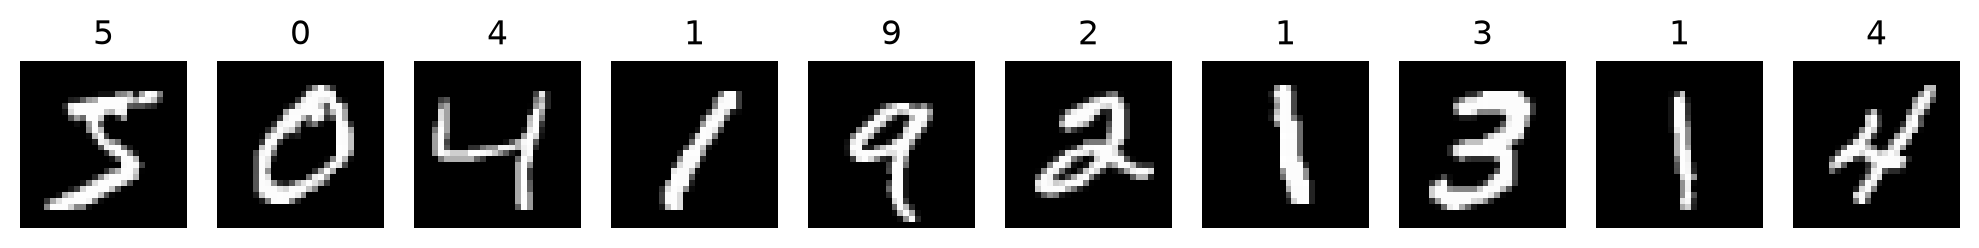
\includegraphics[width=\textwidth]{figures/mnist_samples.png}

\small MNIST 훈련 데이터의 예 (위의 숫자는 정답 label)
\end{center}
}{%
\begin{center}
\fbox{\parbox{0.8\textwidth}{\centering\small
[그림 자리] \texttt{figures/mnist\_samples.png}\\
\texttt{mnist\_lab.py}를 실행하면 생성된다.}}
\end{center}
}

\subsection{Step 2. 계층(layer) 클래스}

각 계층은 \texttt{forward}에서 역전파에 필요한 값을 저장해 두고,
\texttt{backward}에서 upstream gradient를 받아 앞쪽 층으로 보낼 gradient를 돌려준다.

\begin{lstlisting}
class Affine:
    """A = X W + B  for a mini-batch X of shape (h, l)."""
    def __init__(self, W, B):
        self.W = W          # (l, m)
        self.B = B          # (1, m)
        self.X = None
        self.dW = None
        self.dB = None

    def forward(self, X):
        self.X = X
        return X @ self.W + self.B          # (h,l)@(l,m) + (1,m) -> (h, m)

    def backward(self, dA):
        # dA = dL/dA (h, m). It already contains the 1/h of the mini-batch mean,
        # so here we only SUM the contributions of the h samples.
        self.dW = self.X.T @ dA                          # (l,h)@(h,m) -> (l, m)
        self.dB = np.sum(dA, axis=0, keepdims=True)      # sum over rows -> (1, m)
        return dA @ self.W.T                             # dL/dX : (h, l)


class Relu:
    def __init__(self):
        self.mask = None

    def forward(self, A):
        self.mask = (A > 0)                 # True where the node is active
        return np.where(self.mask, A, 0.0)

    def backward(self, dZ):
        return np.where(self.mask, dZ, 0.0) # pass dZ only where A > 0


class Sigmoid:
    def __init__(self):
        self.Z = None

    def forward(self, A):
        self.Z = 1.0 / (1.0 + np.exp(-A))
        return self.Z

    def backward(self, dZ):
        return dZ * self.Z * (1.0 - self.Z)


def softmax(U):
    U = U - np.max(U, axis=1, keepdims=True)   # same result, avoids overflow of exp
    expU = np.exp(U)
    return expU / np.sum(expU, axis=1, keepdims=True)


class SoftmaxWithCrossEntropy:
    def __init__(self):
        self.Y = None
        self.T = None

    def forward(self, U, T):
        self.T = T
        self.Y = softmax(U)                                  # (h, n)
        h = U.shape[0]
        return -np.sum(T * np.log(self.Y + 1e-12)) / h       # mean over the mini-batch

    def backward(self):
        h = self.T.shape[0]
        return (self.Y - self.T) / h        # dL/dU : the ONLY place where we divide by h


class SoftmaxWithSquaredError:
    """Same softmax output, but loss = (1/h) * sum 0.5*(y - t)^2  (for comparison)."""
    def __init__(self):
        self.Y = None
        self.T = None

    def forward(self, U, T):
        self.T = T
        self.Y = softmax(U)
        h = U.shape[0]
        return 0.5 * np.sum((self.Y - self.T) ** 2) / h

    def backward(self):
        h = self.T.shape[0]
        R = self.Y - self.T                                  # dL/dY (times h)
        # multiply by the softmax Jacobian, row by row, without building it
        return self.Y * (R - np.sum(self.Y * R, axis=1, keepdims=True)) / h
\end{lstlisting}

코드와 수식의 대응은 다음과 같다.

\begin{center}
\begin{tabular}{@{}lll@{}}
\toprule
계층 & 수식 & 코드 \\
\midrule
Affine & $\pd{L}{W}=X\T\pd{L}{A}$ & \texttt{X.T @ dA} \\
 & $\pd{L}{B}=\sum_{\text{rows}}\pd{L}{A}$ & \texttt{np.sum(dA, axis=0)} \\
 & $\pd{L}{X}=\pd{L}{A}W\T$ & \texttt{dA @ W.T} \\
ReLU & $\pd{L}{A}=\mathbf{1}[A>0]\odot\pd{L}{Z}$ & \texttt{np.where(mask, dZ, 0)} \\
Sigmoid & $\pd{L}{A}=Z\odot(1-Z)\odot\pd{L}{Z}$ & \texttt{dZ * Z * (1 - Z)} \\
Softmax--CE & $\pd{L}{U}=\frac1h(Y-T)$ & \texttt{(Y - T) / h} \\
Softmax--SE & $\pd{L}{u_i}=\frac1h\,y_i\bigl(r_i-\sum_j y_jr_j\bigr),\ R=Y-T$
& \begin{tabular}[t]{@{}l@{}}\texttt{Y * (R - np.sum(Y * R,}\\ \texttt{\ \ \ \ axis=1, keepdims=True)) / h}\end{tabular} \\
\bottomrule
\end{tabular}
\end{center}

\subsection{Step 3. 2층 신경망 클래스}

\begin{lstlisting}
class TwoLayerNet:
    def __init__(self, input_size, hidden_size, output_size, weight_init_std=0.01,
                 loss="ce"):
        self.params = {
            "W1": weight_init_std * np.random.randn(input_size, hidden_size),
            "B1": np.zeros((1, hidden_size)),
            "W2": weight_init_std * np.random.randn(hidden_size, output_size),
            "B2": np.zeros((1, output_size)),
        }
        self.affine1 = Affine(self.params["W1"], self.params["B1"])
        self.act     = Relu()                    # or Sigmoid()
        self.affine2 = Affine(self.params["W2"], self.params["B2"])
        if loss == "ce":
            self.last = SoftmaxWithCrossEntropy()
        else:                                    # loss == "se"
            self.last = SoftmaxWithSquaredError()

    def predict(self, X):                        # returns the scores U (h, n)
        A = self.affine1.forward(X)
        Z = self.act.forward(A)
        U = self.affine2.forward(Z)
        return U

    def loss(self, X, T):
        U = self.predict(X)
        return self.last.forward(U, T)

    def backward(self):                          # call right after loss()
        dU = self.last.backward()                # (h, n)
        dZ = self.affine2.backward(dU)           # (h, m)
        dA = self.act.backward(dZ)               # (h, m)
        dX = self.affine1.backward(dA)           # (h, l)
        return {"W1": self.affine1.dW, "B1": self.affine1.dB,
                "W2": self.affine2.dW, "B2": self.affine2.dB}

    def accuracy(self, X, T):
        U = self.predict(X)
        return np.mean(np.argmax(U, axis=1) == np.argmax(T, axis=1))
\end{lstlisting}

\begin{itemize}[leftmargin=1.8em]
\item \texttt{backward}는 \ref{sec:summary}절의 역전파 순서를 그대로 코드로 옮긴 것이다.
\item 예측 class는 확률이 가장 큰 class, 즉 \texttt{np.argmax}이다.
softmax는 크기 순서를 바꾸지 않으므로(\ref{sec:softmax}절의 성질 1)) 점수 $U$의 \texttt{argmax}와 같다.
\item \texttt{Affine} 객체는 \texttt{params}의 배열을 \textbf{같은 메모리로} 참조한다.
따라서 업데이트는 \texttt{params[key] -= ...}처럼 제자리(in place)에서 해야 계층에도 반영된다.
\end{itemize}

\subsection{Step 4. 기울기 검사 (gradient check)}

역전파 코드가 맞는지는 \textbf{수치미분}과 비교하여 확인할 수 있다.
작은 network에서 각 parameter를 $\pm\varepsilon$만큼 바꿔 손실의 변화로 미분을 근사한다:
\[
\pd{L}{w}\approx\frac{L(w+\varepsilon)-L(w-\varepsilon)}{2\varepsilon}.
\]

\begin{lstlisting}
def numerical_gradient(f, P, eps=1e-5):
    """Central difference of the scalar function f() w.r.t. every entry of array P."""
    grad = np.zeros_like(P)
    for idx in np.ndindex(P.shape):
        old = P[idx]
        P[idx] = old + eps
        f_plus = f()
        P[idx] = old - eps
        f_minus = f()
        P[idx] = old
        grad[idx] = (f_plus - f_minus) / (2 * eps)
    return grad

X_small = np.random.randn(6, 4)
T_small = np.eye(3)[np.random.randint(0, 3, size=6)]

for loss_type in ["ce", "se"]:
    small = TwoLayerNet(input_size=4, hidden_size=5, output_size=3,
                        weight_init_std=1.0, loss=loss_type)
    small.loss(X_small, T_small)
    grads = small.backward()
    for key in small.params:
        num = numerical_gradient(lambda: small.loss(X_small, T_small), small.params[key])
        print(f"[{loss_type}] {key}: max |backprop - numerical| = "
              f"{np.max(np.abs(grads[key] - num)):.2e}")
\end{lstlisting}

차이가 $10^{-8}$ 이하로 아주 작으면 역전파가 올바르게 구현된 것이다.
(수치미분은 parameter 하나마다 순전파를 두 번 해야 하므로 느리다.
그래서 실제 학습에는 역전파를 쓰고, 수치미분은 \textbf{검증}에만 쓴다.)

\subsection{Step 5. 미니배치 학습}

\begin{lstlisting}
network = TwoLayerNet(input_size=784, hidden_size=100, output_size=10)

epochs        = 10
batch_size    = 100
learning_rate = 0.1

N = x_train.shape[0]
iter_per_epoch = N // batch_size          # 600 iterations = 1 epoch

loss_history   = []
train_acc_list = []
test_acc_list  = []

for epoch in range(epochs):
    perm = np.random.permutation(N)       # shuffle once per epoch
    for it in range(iter_per_epoch):
        idx = perm[it * batch_size:(it + 1) * batch_size]
        X_batch, T_batch = x_train[idx], t_train[idx]

        loss  = network.loss(X_batch, T_batch)   # forward
        grads = network.backward()               # backward
        for key in network.params:               # gradient descent (in place)
            network.params[key] -= learning_rate * grads[key]

        loss_history.append(loss)

    train_acc = network.accuracy(x_train, t_train)
    test_acc  = network.accuracy(x_test, t_test)
    train_acc_list.append(train_acc)
    test_acc_list.append(test_acc)
    print(f"epoch {epoch + 1:2d}: loss={loss:.4f}, "
          f"train acc={train_acc:.4f}, test acc={test_acc:.4f}")
\end{lstlisting}

학습이 끝나면 손실과 정확도의 변화를 그려 \texttt{figures/mnist\_loss\_acc.png}로 저장한다
(그림 그리는 코드는 \texttt{mnist\_lab.py} 참조).

\IfFileExists{figures/mnist_loss_acc.png}{%
\begin{center}
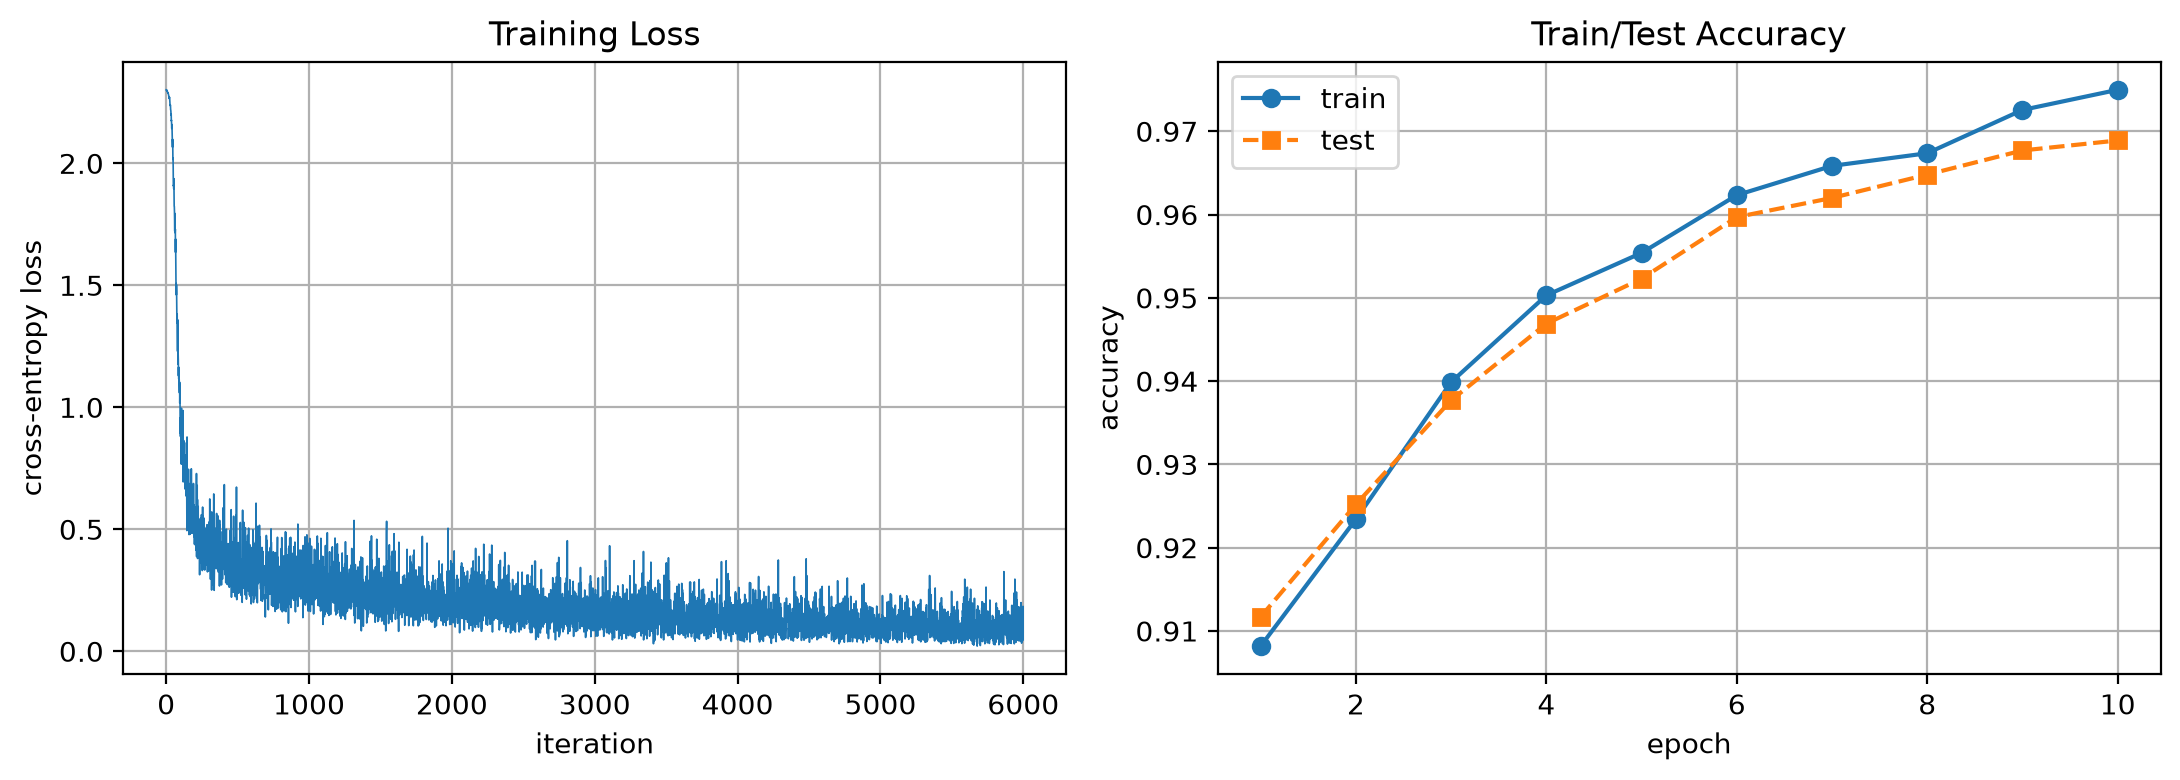
\includegraphics[width=\textwidth]{figures/mnist_loss_acc.png}

\small iteration에 따른 미니배치 손실(왼쪽)과 epoch에 따른 train/test 정확도(오른쪽)
\end{center}
}{%
\begin{center}
\fbox{\parbox{0.8\textwidth}{\centering\small
[그림 자리] \texttt{figures/mnist\_loss\_acc.png}\\
\texttt{mnist\_lab.py}를 실행하면 생성된다.}}
\end{center}
}

\begin{thinkbox}[관찰해 보자]
\begin{itemize}[leftmargin=1.5em]
\item 미니배치 손실 그래프는 왜 매끄럽지 않고 들쭉날쭉한가?
(매 iteration마다 \textbf{다른} $100$개의 데이터로 손실을 계산하기 때문이다.)
\item train 정확도와 test 정확도의 차이는 어느 정도인가?
test 데이터는 학습에 한 번도 쓰이지 않았다는 점을 기억하자.
\item \texttt{learning\_rate}를 $0.01$, $0.5$로, \texttt{batch\_size}를 $10$, $1000$으로 바꾸면
학습 속도와 손실 그래프가 어떻게 달라지는가?
\item \texttt{Relu()}를 \texttt{Sigmoid()}로 바꾸면 어떻게 되는가?
\item \texttt{TwoLayerNet(..., loss="se")}로 제곱 오차를 쓰면 처음 몇 epoch의 정확도가 어떻게 달라지는가?
(\ref{sec:whyce}절)
\end{itemize}
\end{thinkbox}

\subsection{Step 6. 예측 결과 확인}

\begin{lstlisting}
U_test = network.predict(x_test)
Y_test = softmax(U_test)
pred   = np.argmax(Y_test, axis=1)

wrong = np.where(pred != t_test_o)[0]
print("number of wrong predictions:", len(wrong), "/", len(t_test_o))
\end{lstlisting}

\IfFileExists{figures/mnist_predictions.png}{%
\begin{center}
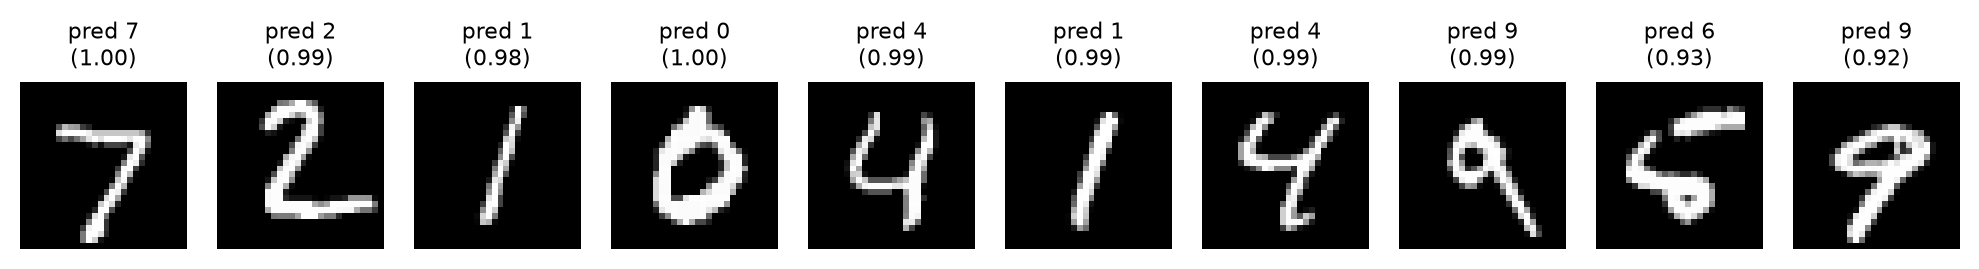
\includegraphics[width=\textwidth]{figures/mnist_predictions.png}

\small test 데이터에 대한 예측 class와 그 확률 $y_k$
\end{center}
}{%
\begin{center}
\fbox{\parbox{0.8\textwidth}{\centering\small
[그림 자리] \texttt{figures/mnist\_predictions.png}\\
\texttt{mnist\_lab.py}를 실행하면 생성된다.}}
\end{center}
}

\IfFileExists{figures/mnist_wrong.png}{%
\begin{center}
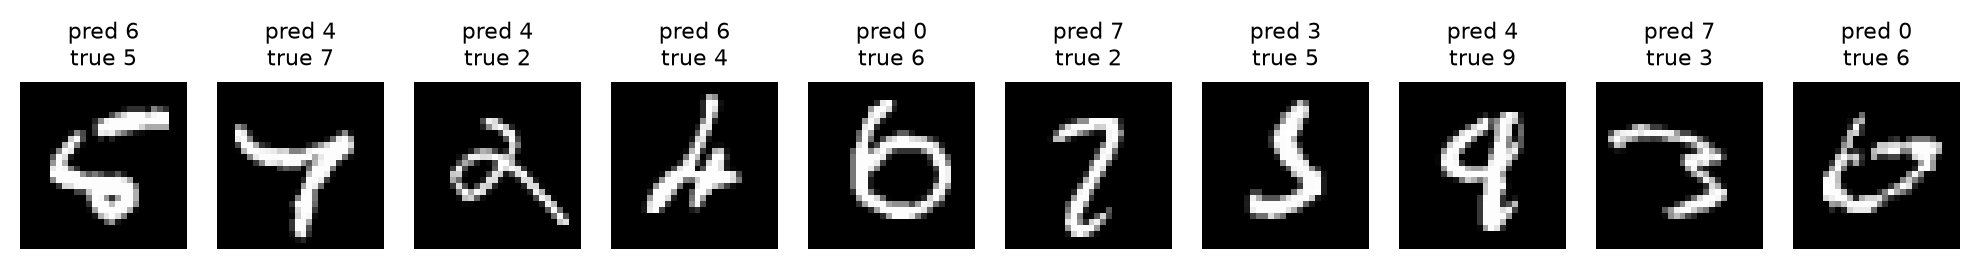
\includegraphics[width=\textwidth]{figures/mnist_wrong.png}

\small 틀리게 예측한 test 데이터의 예 (pred: 예측, true: 정답)
\end{center}
}{%
\begin{center}
\fbox{\parbox{0.8\textwidth}{\centering\small
[그림 자리] \texttt{figures/mnist\_wrong.png}\\
\texttt{mnist\_lab.py}를 실행하면 생성된다.}}
\end{center}
}

틀린 예들을 보면 사람이 보기에도 헷갈리는 숫자가 많다.
network는 각 숫자를 $784$개 픽셀 값의 함수로만 보고 있으며,
픽셀 사이의 공간적 구조(어떤 픽셀이 서로 이웃인지)는 전혀 사용하지 않는다는 점도 생각해 보자.

\subsection{Step 7. 층을 깊이 쌓기: 완전 연결 심층신경망 (\texttt{mnist\_mlp.py})}\label{sec:mlp}

지금까지 만든 network는 affine 계층과 활성화 계층을 한 번 거친 뒤 출력층으로 가는 2층 신경망이었다.
그런데 계층을 클래스로 만들어 두었으므로,
\textbf{affine 계층과 활성화 계층의 조합을 원하는 만큼 반복해서 쌓기만} 하면
은닉층이 여러 개인 network를 바로 만들 수 있다.

\begin{center}
\begin{tikzpicture}[>=Latex,
  lay/.style={draw,rounded corners=2pt,minimum width=11mm,minimum height=24mm,font=\small,fill=softblue},
  act/.style={draw,rounded corners=2pt,minimum width=10mm,minimum height=24mm,font=\small,fill=green!8}]
\node[font=\small] (x) at (0,0) {$X$};
\node[lay] (a1) at (1.3,0) {Affine};
\node[act] (r1) at (2.6,0) {ReLU};
\node[lay] (a2) at (3.9,0) {Affine};
\node[act] (r2) at (5.2,0) {ReLU};
\node (dots) at (6.4,0) {$\cdots$};
\node[lay] (a3) at (7.6,0) {Affine};
\node[act] (r3) at (8.9,0) {ReLU};
\node[lay] (a4) at (10.2,0) {Affine};
\node[draw,rounded corners=2pt,minimum width=14mm,minimum height=24mm,font=\small,fill=orange!12,align=center] (sm) at (11.9,0) {Softmax\\--CE};
\draw[->] (x) -- (a1); \draw[->] (a1) -- (r1); \draw[->] (r1) -- (a2); \draw[->] (a2) -- (r2);
\draw[->] (r2) -- (dots); \draw[->] (dots) -- (a3); \draw[->] (a3) -- (r3); \draw[->] (r3) -- (a4); \draw[->] (a4) -- (sm);
\draw[decorate,decoration={brace,amplitude=5pt,mirror}] (0.75,-1.45) -- (3.15,-1.45)
  node[midway,below=6pt,font=\small] {은닉층 1};
\draw[decorate,decoration={brace,amplitude=5pt,mirror}] (3.35,-1.45) -- (5.75,-1.45)
  node[midway,below=6pt,font=\small] {은닉층 2};
\draw[decorate,decoration={brace,amplitude=5pt,mirror}] (7.05,-1.45) -- (9.45,-1.45)
  node[midway,below=6pt,font=\small] {은닉층 $k$};
\draw[decorate,decoration={brace,amplitude=5pt,mirror}] (9.65,-1.45) -- (12.65,-1.45)
  node[midway,below=6pt,font=\small] {출력층};
\end{tikzpicture}
\end{center}

각 affine 계층에서는 앞 층의 \textbf{모든} node가 다음 층의 \textbf{모든} node와 가중치로 연결되어 있다.
이렇게 affine 계층과 활성화 계층을 반복해 쌓은 network를
\textbf{완전 연결 신경망(fully connected neural network)} 또는 \textbf{다층 퍼셉트론(multi-layer perceptron, MLP)}이라 하고,
은닉층이 여러 개이면 \textbf{완전 연결 심층신경망}이라 한다.

\begin{keybox}[깊이와 넓이로 표현력을 키운다]
지난주에 hidden neuron을 늘리면 더 복잡한 함수를 근사할 수 있음을 보았다 (universal approximation).
마찬가지로
\begin{itemize}[leftmargin=1.8em]
\item 은닉층의 \textbf{넓이}(node 수)를 늘리거나,
\item 은닉층의 \textbf{깊이}(층 수)를 늘려 앞 층이 만든 특징을 다시 조합하게 하면,
\end{itemize}
network가 표현할 수 있는 함수가 풍부해지고 분류 성능이 좋아질 수 있다.
network 구조를 바꾸는 것만으로도, 즉 \textbf{깊이와 넓이의 조정만으로도} 성능을 끌어올릴 수 있다.
단, parameter가 많아질수록 훈련 데이터에만 지나치게 맞추는 \textbf{과적합}의 위험도 커진다.
\end{keybox}

새 계층을 만들 필요는 없다. \texttt{mnist\_mlp.py}의 \texttt{MultiLayerNet}은
\texttt{mnist\_lab.py}와 \textbf{똑같은} \texttt{Affine}, \texttt{Relu}, \texttt{Sigmoid}, softmax 계층을
리스트에 차례로 담아 쌓을 뿐이다.

\begin{lstlisting}
class MultiLayerNet:
    def __init__(self, input_size, hidden_sizes, output_size,
                 activation="relu", loss="ce", weight_init_std=0.05):
        sizes = [input_size] + list(hidden_sizes) + [output_size]   # e.g. [784, 256, 128, 10]
        self.params = {}
        self.layers = []
        for i in range(len(sizes) - 1):
            n_in, n_out = sizes[i], sizes[i + 1]
            W = weight_init_std * np.random.randn(n_in, n_out)   # (input nodes, output nodes)
            B = np.zeros((1, n_out))
            self.params[f"W{i + 1}"] = W
            self.params[f"B{i + 1}"] = B
            self.layers.append(Affine(W, B))
            if i < len(sizes) - 2:                     # no activation after the last Affine
                self.layers.append(Relu() if activation == "relu" else Sigmoid())
        self.last = SoftmaxWithCrossEntropy() if loss == "ce" else SoftmaxWithSquaredError()

    def predict(self, X):                     # scores U
        for layer in self.layers:
            X = layer.forward(X)
        return X

    def loss(self, X, T):
        return self.last.forward(self.predict(X), T)

    def backward(self):                       # call right after loss()
        d = self.last.backward()
        for layer in reversed(self.layers):   # the same rule, layer after layer
            d = layer.backward(d)
        grads, k = {}, 1
        for layer in self.layers:
            if isinstance(layer, Affine):
                grads[f"W{k}"], grads[f"B{k}"] = layer.dW, layer.dB
                k += 1
        return grads
\end{lstlisting}

\begin{itemize}[leftmargin=1.8em]
\item \texttt{hidden\_sizes}는 은닉층들의 넓이를 담은 리스트이다. 예를 들어
\begin{lstlisting}
net = MultiLayerNet(784, [256, 128], 10)
\end{lstlisting}
은 넓이가 $256$, $128$인 은닉층 두 개를 가진 \textbf{3층} 신경망이다.
\item 순전파는 계층 목록을 앞에서부터, 역전파는 \textbf{거꾸로} 돌며 각 계층의 \texttt{backward}를 호출한다.
층이 몇 개이든 이번 주에 유도한 규칙을 반복할 뿐이다.
\item 가중치는 모두 표준편차 \texttt{weight\_init\_std}$=0.05$인 정규분포로 초기화한다.
층이 깊어질 때 가중치를 어떻게 초기화해야 학습이 잘 되는지는 다음 주에 다룬다.
\end{itemize}

\subsection*{훈련 / 검증 / test 데이터}

여러 network 중 어느 것이 좋은지를 고를 때 test 데이터를 보면 안 된다.
test 정확도를 보면서 설정을 고르면, test 데이터에 맞춰 설정을 고른 셈이 되어
처음 보는 데이터에 대한 성능을 과대평가하게 된다.
그래서 \texttt{mnist\_mlp.py}는 훈련 데이터 $60000$개 중 $5000$개를 떼어 \textbf{검증(validation) 데이터}로 두고,
\begin{enumerate}[leftmargin=1.8em]
\item 나머지 $55000$개로 학습하고,
\item 여러 설정을 \textbf{검증 정확도}로 비교하여 가장 좋은 것을 고른 뒤,
\item 고른 network의 성능을 test 데이터로 \textbf{단 한 번} 평가한다.
\end{enumerate}

\subsection*{실험하는 방법}

실험할 설정은 \texttt{mnist\_mlp.py}의 \texttt{experiments} 리스트에 한 줄씩 적는다.

\begin{lstlisting}
# Edit this list for Assignment 2. Each line is one experiment:
#   (name, hidden layer widths, activation, loss, learning rate, batch size)
# Change ONE thing at a time and compare the validation accuracy.
experiments = [
    ("A: [100]",      [100],      "relu", "ce", 0.1, 100),   # the network of the lab (Step 5)
    ("B: [100, 100]", [100, 100], "relu", "ce", 0.1, 100),   # one more hidden layer
]
epochs = 10
\end{lstlisting}

실행하면 각 설정의 epoch별 train/검증 정확도가 출력되고, \texttt{figures} 폴더에 그림 두 개가 저장된다.
\begin{itemize}[leftmargin=1.8em]
\item \texttt{mlp\_compare.png}: 설정들의 epoch별 정확도 비교 그래프
\item \texttt{mlp\_confusion.png}: 검증 정확도가 가장 높은 network의 test 혼동행렬
\end{itemize}
\textbf{혼동행렬(confusion matrix)}의 $i$행 $j$열은 ``정답이 $i$인데 $j$로 예측한 test 이미지의 개수''이며,
대각선이 맞힌 개수이다.

\begin{thinkbox}[과제 2를 시작하며 생각해 볼 질문]
\begin{itemize}[leftmargin=1.5em]
\item 은닉층을 넓게 하는 것과 깊게 쌓는 것 중 어느 쪽이 더 효과적인가?
parameter 수가 비슷하도록 맞춰서 비교해 보라 (\texttt{num\_params()}).
\item train 정확도와 검증 정확도의 차이는 network가 커질수록 어떻게 변하는가?
\item 학습률과 미니배치 크기를 바꾸면 손실 그래프와 정확도는 어떻게 달라지는가?
\item ReLU 대신 sigmoid를, cross entropy 대신 제곱 오차를 쓰면 어떻게 되는가?
\item 혼동행렬에서 가장 많이 헷갈린 숫자 쌍은 무엇인가?
\end{itemize}
\end{thinkbox}


% =================================================
\section{이번 주의 핵심 정리}
% =================================================

\begin{keybox}[핵심 구조]
다차원 다중분류 network:
\[
\boxed{
A=XW^{(1)}+B^{(1)},\ \ Z=h(A),\ \ U=ZW^{(2)}+B^{(2)},\ \ Y=\softmax(U)
}
\]
\[
\boxed{
l=-\sum_i t_i\log y_i
}
\]

Affine 계층의 역전파 (한 데이터든 미니배치든 같은 식):
\[
\boxed{
\pd{L}{X}=\pd{L}{A}W\T,\qquad \pd{L}{W}=X\T\pd{L}{A},\qquad \pd{L}{B}=\texttt{np.sum}\Bigl(\pd{L}{A},\ \texttt{axis=0}\Bigr)
}
\]

활성화 계층의 역전파는 성분별 곱:
\[
\boxed{
\pd{L}{A}=h'(A)\odot\pd{L}{Z}
}
\qquad(\text{ReLU: }\mathbf{1}[A>0],\ \ \text{sigmoid: }Z\odot(1-Z))
\]

Softmax--cross entropy:
\[
\boxed{
\pd{l}{U}=Y-t
}
\qquad(\text{미니배치 평균이면 }\tfrac1h(Y-T))
\]

미니배치 학습:
\[
\boxed{
\text{평균은 손실에서 한 번만},\quad \text{데이터에 대한 합은 행렬곱과 axis=0의 합}
}
\]
\end{keybox}

% =================================================
\section{연습문제}
% =================================================

\begin{enumerate}[label=\arabic*.]

\item MNIST network에서 $l=784$, $m=100$, $n=10$, 미니배치 크기 $h=100$이다.
$X$, $W^{(1)}$, $B^{(1)}$, $A$, $Z$, $W^{(2)}$, $B^{(2)}$, $U$, $Y$, $T$의 shape을 쓰고,
학습해야 하는 parameter의 총 개수를 구하라.

\item $U=(1,2,3)$일 때 $Y=\softmax(U)$를 소수 셋째 자리까지 구하라.
또 임의의 상수 $c$에 대하여 $\softmax(U+c)=\softmax(U)$임을 보이라.

\item 정답이 $t=(0,0,1)$이고 network의 출력이 $Y=(0.2,\,0.3,\,0.5)$일 때
cross entropy 손실 $l$과 $\pd{l}{U}$를 구하라.
경사하강법은 세 점수 $u_1,u_2,u_3$를 각각 어느 방향으로 움직이는가?

\item Affine 계층 $A=XW+B$에서
\[
X=(1,\ 2),\qquad
W=\begin{pmatrix}1&0&-1\\2&1&0\end{pmatrix},\qquad
B=(0,\ 1,\ 0),\qquad
\pd{l}{A}=(1,\ -1,\ 2)
\]
일 때 $A$, $\pd{l}{X}$, $\pd{l}{W}$, $\pd{l}{B}$를 구하라.

\item softmax의 Jacobian $J=\left(\pd{y_j}{u_i}\right)$가
\[
J=\operatorname{diag}(y_1,\ldots,y_n)-Y\T Y
\]
로 쓸 수 있음을 보이라. ($Y$는 $1\times n$ 행벡터)

\item ReLU 계층의 역전파를 다음과 같이 구현한 코드가 있다.
\begin{lstlisting}
def backward(self, dZ):
    return np.maximum(self.A, 0) * dZ
\end{lstlisting}
무엇이 잘못되었는지 설명하고 올바르게 고쳐라.

\item 미니배치 학습에서 softmax--CE 계층이 \texttt{(Y - T) / h}를 돌려주는데,
affine 계층의 \texttt{backward}에서도 \texttt{self.dW = self.X.T @ dA / h}처럼 다시 $h$로 나누었다고 하자.
$\pd{L}{W^{(2)}}$와 $\pd{L}{W^{(1)}}$는 정확한 값의 몇 배가 되는가?

\item (도전) 손실함수를 제곱 손실 $l=\frac12\sum_i(y_i-t_i)^2$으로 바꾸면
\[
\pd{l}{u_i}=y_i\Bigl((y_i-t_i)-\sum_{j=1}^{n}y_j(y_j-t_j)\Bigr)
\]
임을 보이라 (\ref{sec:whyce}절). 또 $R=Y-T$라 할 때 이 식을 미니배치 행렬로 쓰면
\begin{lstlisting}
Y * (R - np.sum(Y * R, axis=1, keepdims=True))
\end{lstlisting}
가 됨을 확인하라.

\end{enumerate}

% =================================================
\section{과제}
% =================================================

\subsection*{XOR 문제}

XOR 문제는 인공지능과 신경망에서 비선형 분류 문제의 대표적인 예제로,
신경망의 학습 능력을 설명할 때 자주 사용되는 문제이다.
XOR(배타적 논리합)은 \textbf{두 입력이 다를 때만 출력이 1}이 되는 이진 연산 문제로서
다음과 같이 표와 그림으로 설명할 수 있다.

\begin{center}
\begin{minipage}{0.58\textwidth}
\centering
\begin{tabular}{|c|c|c|}
\hline
\begin{tabular}{@{}c@{}}입력\\ $X_i=(x_1,x_2)$\end{tabular} & 정답, 레이블 &
\begin{tabular}{@{}c@{}}원핫벡터\\ $t_i=(t_1,t_2)$\end{tabular} \\
\hline
$(0,0)$ & $0$ & $(1,0)$ \\ \hline
$(1,0)$ & $1$ & $(0,1)$ \\ \hline
$(0,1)$ & $1$ & $(0,1)$ \\ \hline
$(1,1)$ & $0$ & $(1,0)$ \\ \hline
\end{tabular}
\end{minipage}
\hfill
\begin{minipage}{0.36\textwidth}
\centering
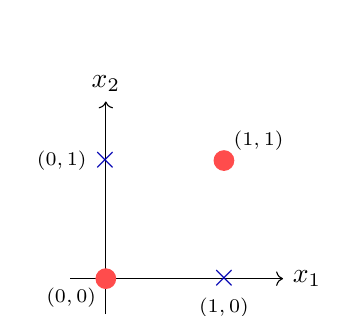
\begin{tikzpicture}[scale=1.5]
\draw[->] (-0.3,0) -- (1.5,0) node[right] {$x_1$};
\draw[->] (0,-0.3) -- (0,1.5) node[above] {$x_2$};
\foreach \p in {(0,0),(1,1)} \fill[red!70] \p circle (2.5pt);
\foreach \p in {(1,0),(0,1)} \node[blue!70!black,font=\large] at \p {$\times$};
\node[below left,font=\scriptsize] at (0,0) {$(0,0)$};
\node[below,font=\scriptsize] at (1,-0.08) {$(1,0)$};
\node[left,font=\scriptsize] at (-0.08,1) {$(0,1)$};
\node[above right,font=\scriptsize] at (1,1) {$(1,1)$};
\end{tikzpicture}
\end{minipage}
\end{center}

위와 같이 두 입력 $x_1$, $x_2$가 다를 때에는 $1$을 출력하고, 같을 때에는 $0$을 출력하는 문제인데,
이것을 이차원 평면에 나타내면 네 개의 점을 두 개의 그룹으로 나누는 것이다.
XOR 문제는 인공지능, 특히 신경망(neural networks) 연구의 역사에서 중요한 전환점을 나타내는 문제인데,
이 간단한 논리 연산이 AI 발전의 중단과 부흥을 모두 상징하는 사례로 여겨지는 이유는 다음과 같다.

1958년 로젠블랫이 퍼셉트론(perceptron)을 제안하면서 최초의 인공신경망의 개념이 탄생하였다.
퍼셉트론이란 은닉층이 없는 신경망으로 입력층에서 신호를 받아 활성화 함수를 거쳐 값을 출력하는 단순한 신경망을 말한다.
로젠블랫은 퍼셉트론을 학습시키는 알고리즘을 제시하였고
이로써 기계학습이 세상의 모든 문제를 해결할 수 있으리라는 기대감에
인공지능에 대한 연구는 큰 부흥기를 맞으며 천문학적인 연구 예산이 투입된다.
그러나 이후 단순히 퍼셉트론으로는 XOR 문제를 풀 수 없다는 것을 민스키와 페퍼트가 증명하면서,
인공지능의 첫 번째 겨울이 찾아왔다.
당시 민스키와 페퍼트를 비롯한 사람들은 XOR 문제를 여러 개의 퍼셉트론을 계층적으로 연결한 신경망,
즉 은닉층이 있는 다층 신경망(Multi-Layer Perceptron, MLP)으로 구현할 수 있을 것이란 것은 알고는 있었지만,
그러한 다층 신경망을 훈련하는 알고리즘은 존재하지 않을 것으로 여겼기 때문에
인공신경망에 대한 연구가 암흑기를 맞이한다.
이후 1986년에 David Rumelhart, Geoffrey Hinton, Ronald Williams가 다층 신경망을 훈련하는 알고리즘을 개발하였는데,
바로 이것이 경사하강법과 합성함수 미분법을 바탕으로 한 역전파(backpropagation) 알고리즘이다.
은닉층이 하나 이상일 때 신경망을 훈련하는 방법이 완성되면서 인공지능이 다시 부흥기로 들어서게 되었고,
수많은 은닉층을 갖는 인공신경망, 즉 심층신경망(Deep Neural Network, DNN)을 활용한 연구가 다시 부흥기를 맞이한다.

\subsection*{과제 1. XOR 문제의 온라인 학습을 손으로 계산하기}

XOR 문제를 은닉층이 1개이고 출력층에 softmax를 사용하는 다음과 같은 신경망으로 학습시키는 과정을 연습해 보자.

다음과 같이 변수를 정의하자.
\[
X=(x_1,x_2):\ \text{입력 데이터},
\qquad
t=(t_1,t_2):\ \text{정답 레이블의 원핫 인코딩}
\]
\[
A=(a_1,a_2),\quad Z=(z_1,z_2),\quad U=(u_1,u_2),\quad Y=(y_1,y_2).
\]

\begin{center}
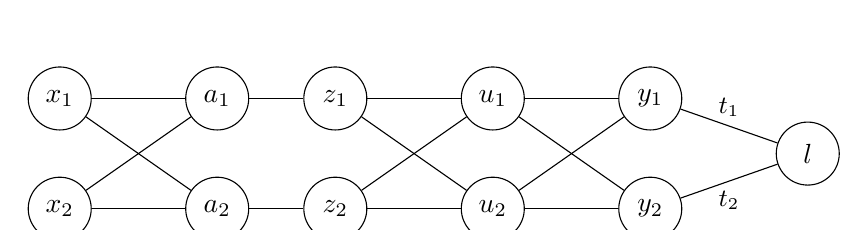
\begin{tikzpicture}[>=Latex,
  nd/.style={draw,circle,minimum size=8mm,inner sep=0pt}]
\node[nd] (x1) at (0,0.7) {$x_1$};  \node[nd] (x2) at (0,-0.7) {$x_2$};
\node[nd] (a1) at (2,0.7) {$a_1$};  \node[nd] (a2) at (2,-0.7) {$a_2$};
\node[nd] (z1) at (3.5,0.7) {$z_1$};  \node[nd] (z2) at (3.5,-0.7) {$z_2$};
\node[nd] (u1) at (5.5,0.7) {$u_1$};  \node[nd] (u2) at (5.5,-0.7) {$u_2$};
\node[nd] (y1) at (7.5,0.7) {$y_1$};  \node[nd] (y2) at (7.5,-0.7) {$y_2$};
\node[nd] (l) at (9.5,0) {$l$};
\foreach \i in {x1,x2} \foreach \j in {a1,a2} \draw (\i) -- (\j);
\draw (a1) -- (z1); \draw (a2) -- (z2);
\foreach \i in {z1,z2} \foreach \j in {u1,u2} \draw (\i) -- (\j);
\foreach \i in {u1,u2} \foreach \j in {y1,y2} \draw (\i) -- (\j);
\draw (y1) -- node[above,font=\small] {$t_1$} (l);
\draw (y2) -- node[below,font=\small] {$t_2$} (l);
\end{tikzpicture}
\end{center}

가중치와 편이를
\[
W^{(1)}=\begin{pmatrix}w^{(1)}_{11}&w^{(1)}_{12}\\ w^{(1)}_{21}&w^{(1)}_{22}\end{pmatrix},\quad
B^{(1)}=\bigl(b^{(1)}_1,b^{(1)}_2\bigr),\quad
W^{(2)}=\begin{pmatrix}w^{(2)}_{11}&w^{(2)}_{12}\\ w^{(2)}_{21}&w^{(2)}_{22}\end{pmatrix},\quad
B^{(2)}=\bigl(b^{(2)}_1,b^{(2)}_2\bigr)
\]
라 하고, 신경망의 순전파를
\[
A=XW^{(1)}+B^{(1)},\quad Z=h(A),\quad U=ZW^{(2)}+B^{(2)},\quad Y=\softmax(U),\quad
l=-\sum_{i=1}^{2}t_i\log y_i
\]
로 정의하자. 초기 가중치와 편이가
\[
W^{(1)}_0=\begin{pmatrix}2&-1\\-2&2\end{pmatrix},\quad
B^{(1)}_0=(1,0),\quad
W^{(2)}_0=\begin{pmatrix}-1&1\\-2&2\end{pmatrix},\quad
B^{(2)}_0=(1,-1)
\]
로 설정되었을 때, 데이터 $X_4=(1,1)$, $t_4=(1,0)$에 대한 온라인 학습을 진행하여 가중치를 업데이트하여라.
이때 $h(x)=\begin{cases}x,&x\ge0\\0,&x<0\end{cases}$로 ReLU 함수를 사용하고, 학습률은 $1$로 계산하고,
실습 코드의 계층 클래스를 활용하여 계산 결과를 확인하여라.

\subsection*{과제 2. MNIST 정확도 98\% 도전}

MNIST 숫자 분류 문제를 실습 코드 \texttt{mnist\_mlp.py}(\ref{sec:mlp}절)를 활용하여 연습하여라.
은닉층의 수(깊이), 은닉층의 노드의 수(넓이), 활성화 함수의 종류, 손실함수의 종류,
학습률, 미니배치 크기, epoch 수 등을 조정하여 테스트 데이터에 대한 정확도를 98\% 이상으로 훈련시켜라.
\begin{itemize}[leftmargin=1.8em]
\item 설정은 \textbf{검증 정확도}로 비교하여 고르고, test 정확도는 최종 선택한 network에 대해서만 보고하라.
\item 한 번에 \textbf{한 가지 요인만} 바꾸어 실험하고,
시도한 설정과 그 결과(train/검증 정확도, 그래프)를 표로 정리하라.
\item 어떤 요인이 정확도에 가장 큰 영향을 주었는지, 과적합의 징후가 있었는지 설명하라.
\end{itemize}

% =================================================
\section*{다음 주 예고}
% =================================================

이번 주에는 은닉층이 1개인 network를 계층(layer) 단위로 구현하였다.
같은 \texttt{Affine}과 활성화 계층을 여러 번 쌓으면 은닉층이 여러 개인 \textbf{심층신경망}이 된다.
다음에는 층이 깊어질 때 학습이 잘 되도록 하는 방법
(최적화 기법, 가중치 초기화, 오버피팅, 드롭아웃 등)을 다룬다.

\vfill

\end{document}
